\documentclass[paper=a4, fontsize=11pt, onecolumn, tikz, dvipsnames, svgnames, x11names]{article}
\usepackage[utf8]{inputenc}
\usepackage[T1]{fontenc}
\usepackage[english]{babel}
\usepackage{multicol}
\usepackage{fullpage}
% ------------------------- Color table ----------------------------------------
\usepackage{multirow}
\usepackage[table]{xcolor}
\definecolor{maroon}{cmyk}{0,0.87,0.68,0.32}
\usepackage{booktabs} % to make prettier tables (toprule, midrule, bottomrule)
% ------------------------------------------------------------------------------

\usepackage{amscd}
\usepackage{amsthm}
\usepackage{physics}
\usepackage{textcomp,gensymb} %pour le °C, et textcomp pour éviter les warning
\usepackage{graphicx} %pour les images
\usepackage{caption}
\usepackage{subcaption}
\usepackage[colorlinks=true,
	breaklinks=true,
	citecolor=blue,
	linkcolor=blue,
	urlcolor=blue]{hyperref} % pour insérer des liens
\usepackage{epstopdf} %converting to PDF
\usepackage[export]{adjustbox} %for large figures

\usepackage{array}
\usepackage{dsfont}% indicatrice : \mathds{1}


% -------------------------- Mathematics ---------------------------------------
\graphicspath{{images/}{../images/}} % For the images path
% ------------------------------------------------------------------------------

% -------------------------- Mathematics ---------------------------------------
\usepackage{mathrsfs, amsmath, amsfonts, amssymb}
\usepackage{bm}
\usepackage{mathtools}
\usepackage[Symbol]{upgreek} % For pi \uppi different from /pi
\newcommand{\R}{\mathbb{R}} % For Real space
\usepackage{tikz}
\usetikzlibrary{bayesnet} %library to draw graphical models1
% ------------------------------------------------------------------------------


% -------------------------- Code format ---------------------------------------
\usepackage[numbered,framed]{matlab-prettifier}
\lstset{
	style              = Matlab-editor,
	basicstyle         = \mlttfamily,
	escapechar         = '',
	mlshowsectionrules = true,
}
% ------------------------------------------------------------------------------

% ------------------------- Blbiographie --------------------------------------
% \usepackage[backend=biber, style=ieee]{biblatex}
% \addbibresource{biblio.bib}
% \bibliography{../material/biblio.bib}
% \usepackage{csquotes}
% ------------------------------------------------------------------------------


\setcounter{tocdepth}{4} %Count paragraph
\setcounter{secnumdepth}{4} %Count paragraph
\usepackage{float}

\usepackage{graphicx} % for graphicspath
% \graphicspath{{../images/}}

\usepackage{array,tabularx}
\newcolumntype{L}[1]{>{\raggedright\let\newline\\\arraybackslash\hspace{0pt}}m{#1}}
\newcolumntype{C}[1]{>{\centering\let\newline\\\arraybackslash\hspace{0pt}}m{#1}}
\newcolumntype{R}[1]{>{\raggedleft\let\newline\\\arraybackslash\hspace{0pt}}m{#1}}


% \usepackage{algpseudocode}
% \usepackage{algorithm}
\usepackage{hyperref}
\usepackage[edges]{forest}

% ------------------------------ Jules packages --------------------------------
\usepackage[ruled,vlined]{algorithm2e}
\usepackage[colorinlistoftodos]{todonotes}
\usepackage{alltt}

% Independent sign
\newcommand{\indep}{\ensuremath{\,\bot\!\!\!\bot\,}} %% The symbol for independent

% Alpha / Numbers for sections
\renewcommand{\thesubsubsection}{\arabic{section}.\arabic{subsection}.\alph{subsubsection})}

\newcommand{\argmin}[1]{\underset{#1}{\operatorname{argmin}}\;}

% % Norm
% \newcommand{\norm}[1]{\left\lVert#1\right\rVert}


% ------------------------ General informations --------------------------------
\title{\normalfont \normalsize \huge Pointing error correction}
\author{Jules Kozolinsky, Vincent Matthys}
\graphicspath{{images/}{../images/}} % For the images path
% ------------------------------------------------------------------------------


\date{}

\begin{document}
%\maketitle

 \begin{tabularx}{0.9\textwidth}{@{} l X r @{} }
 	{\textsc{Master MVA}}  &  & \textsc{} \\
 	\textsc{Remote sensing} &  & {ENS Paris Saclay}       \\
 \end{tabularx}
 \vspace{1.5cm}
 \begin{center}

 	\rule[11pt]{5cm}{0.5pt}

 	\textbf{\LARGE \textsc{Pointing error correction}}
 	\vspace{0.5cm}

 	Jules Kozolinsky,
 	Vincent Matthys

 	\href{mailto:jules.kozolinsky@ens-cachan.fr}{jules.kozolinsky@ens-cachan.fr} \\
 	\href{mailto:vincent.matthys@ens-paris-saclay.fr}{vincent.matthys@ens-paris-saclay.fr}

 	\rule{5cm}{0.5pt}

 	\vspace{1.5cm}
 \end{center}

 \tableofcontents


\section{Satellite imagery}
\subsection{Localization and projection functions}
We define here the localization and projection functions which allow to convert image coordinates to coordinates
on the globe and back (See Figure \ref{rpc}).\\


The projection function returns the image coordinates, in pixels, of a given 3-space
point.
\begin{align*}
P:&\; \mathbb{R}^3\to\mathbb{R}^2\\
&(\lambda, \theta, h) \mapsto \textbf{x}
\end{align*}
In that system, a point of 3-space is identified by its
longitude $\lambda\in[-180,180]$, latitude $\theta\in[-90,90]$ and
altitude $h$, in meters, above the reference ellipsoid.\\


The localization function is its
inverse with respect to the first two components. It takes a point $\textbf{x}
= (x, y)^\top$ in the image domain together with an altitude $h$, and
returns the geographic coordinates of the unique 3-space point
$\textbf{X} = (\lambda, \theta, h)$ whose altitude is $h$ and whose image is $\textbf{x}$.
\begin{align*}
L:&\; \mathbb{R}^3\to\mathbb{R}^2\\
&(\textbf{x}, h) \mapsto (\lambda, \theta)
\end{align*}\\



We use the Rational Polynomial Coefficient (RPC) camera model which is an
analytic description of the projection and localization functions (cite). In the RPC model, the projection and
localization functions are expressed as ratio of multivariate cubic
polynomials.

\begin{figure}[h]
    \centering
    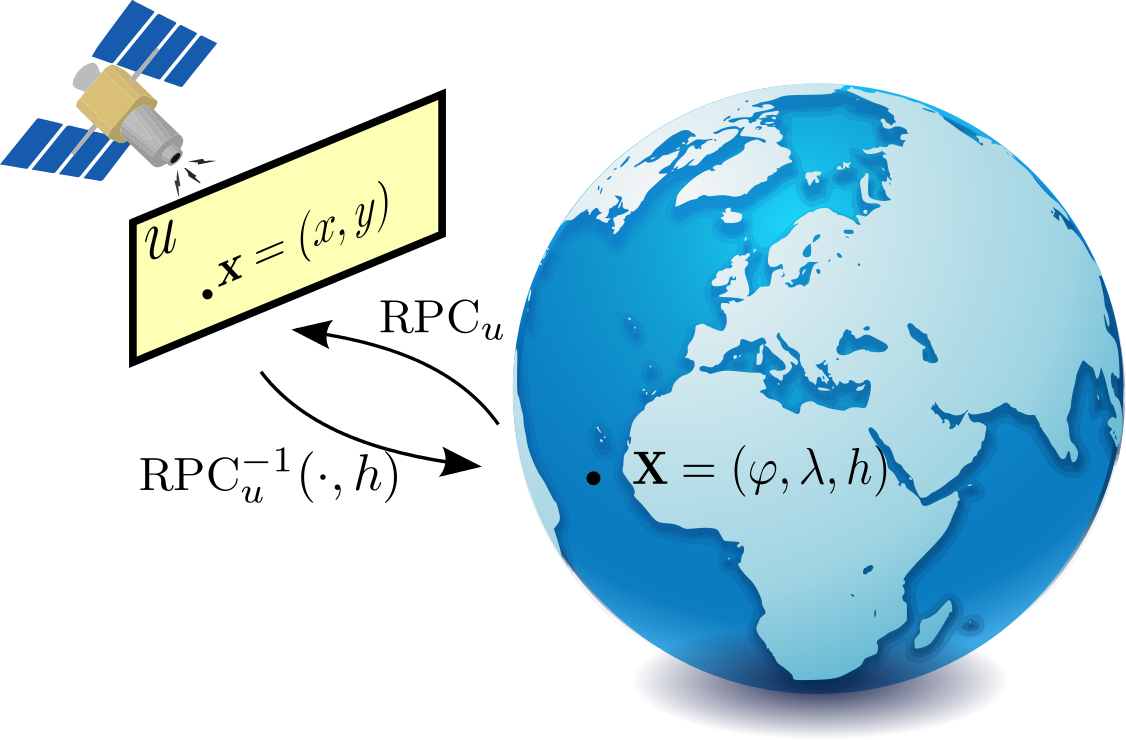
\includegraphics[width=0.5\textwidth]{figures/rpc_illustration.png}
   \caption{ Projection (RPC) and localization (RPC$^{-1}$) functions.}
   \label{rpc}
\end{figure}

\subsection{Epipolar curves}
For a point $\textbf{x}$ in the image $u$, the epipolar curve is the curve pararametrized by the alitude $h$ and defined as:
\begin{align*}
\text{epi}_{uv}^{\textbf{x}} : h \rightarrow \text{RPC}_u(\text{RPC}^{-1}_v(\textbf{x}, h))
\end{align*}
where RPC and RPC$^{-1}$ are the projection and localization functions. In pratice we observe this curve as straight parallel lines.

\subsection{Affine fundamental matrix approximation}
From  \cite{carlo_2014_pushbroom}, we know that, for each point $\textbf{x}_i$, the epipolar curve $\text{epi}^{\textbf{x}_i}_{u v}(R)$ is approximated up to $0.05$ pixels by the straight line $F\textbf{x}_i$, where $F$ is
the affine fundamental matrix between the two views. Since the fundamental matrix, due to the approximation, is \textit{affine}, all the lines $(F\textbf{x}_i)_{i=1...N}$ are parallel.

\section{Satellite attitude error effects on stereo images}
\subsection{Pointing error}
However, due to the limited precision of the
camera calibration, there can be a bias of a few pixels in the RPC functions.
For stereo matching, we can not ignore this error since the epipolar constraints are derived from
the parameters of the cameras.
Therefore this bias has to be corrected before applying rectification.\\

This error, often of the order of a few pixels, is the sum, for all correspondences $(\textbf{x}_i, \textbf{x}'_i)_{i=1...N}$, of the distance between the point $\textbf{x}'_i$ on the left image and the epipolar curve on the left image, computed from the correspondance $\textbf{x}_i$ of the right image.
Formally, given two images $u, v$ and a set of correspondences $(\textbf{x}_i, \textbf{x}'_i)_{i=1...N}$ , the pointing error between $u$ and $v$ is defined by:
\begin{align*}
\dfrac{1}{N} \sum\limits_{i=1}^{N} d(\textbf{x}_i', \text{epi}_{uv}^{\textbf{x}_i})
\end{align*}
which can be approximated, using the affine fundamental matrix $F$, to:
\begin{align*}
\dfrac{1}{N} \sum\limits_{i=1}^{N} d(\textbf{x}_i', F\textbf{x}_i)
\end{align*}

\subsection{Attitude of a Satellite}
The attitude of a satellite refers to the orientation of a three-dimensional coordinate system linked to the satellite with respect to another coordinate system (Earth for example).
We define the roll, pitch and yaw angles as in Figure \ref{angles}.

\begin{figure}[h]
    \centering
    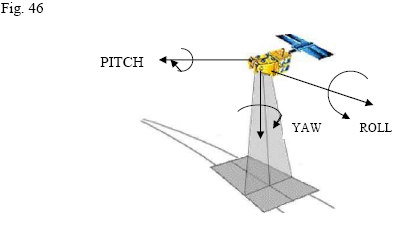
\includegraphics[width=0.5\textwidth]{figures/angles.jpg}
   \caption{ Roll, pitch and yaw angles.}
   \label{angles}
\end{figure}


\subsection{Sensibility}
\label{subsec:sensibility}
%Sensiblity of roll, pitch and yaw. Scheme (roll and pitch depend of the height of the satellite whereas yaw only the angle)
The effect of attitude errors on the localization function RPC$^{-1}$ can be computed simply with zero roll and pitch angles. For roll or pitch angles
a small error $\varepsilon$ induces, to first order, a translation of $a\varepsilon$ on the ground, where $a$ is
the distance between the satellite and the ground. For the yaw, a small error $\varepsilon$  induces
a rotation of at most $D\varepsilon/2$ on the ground, where $D$ is the width of the projected pushbroom sensor of the satellite (See Figure \ref{sensiblity}).

\begin{figure}[h]
    \centering
    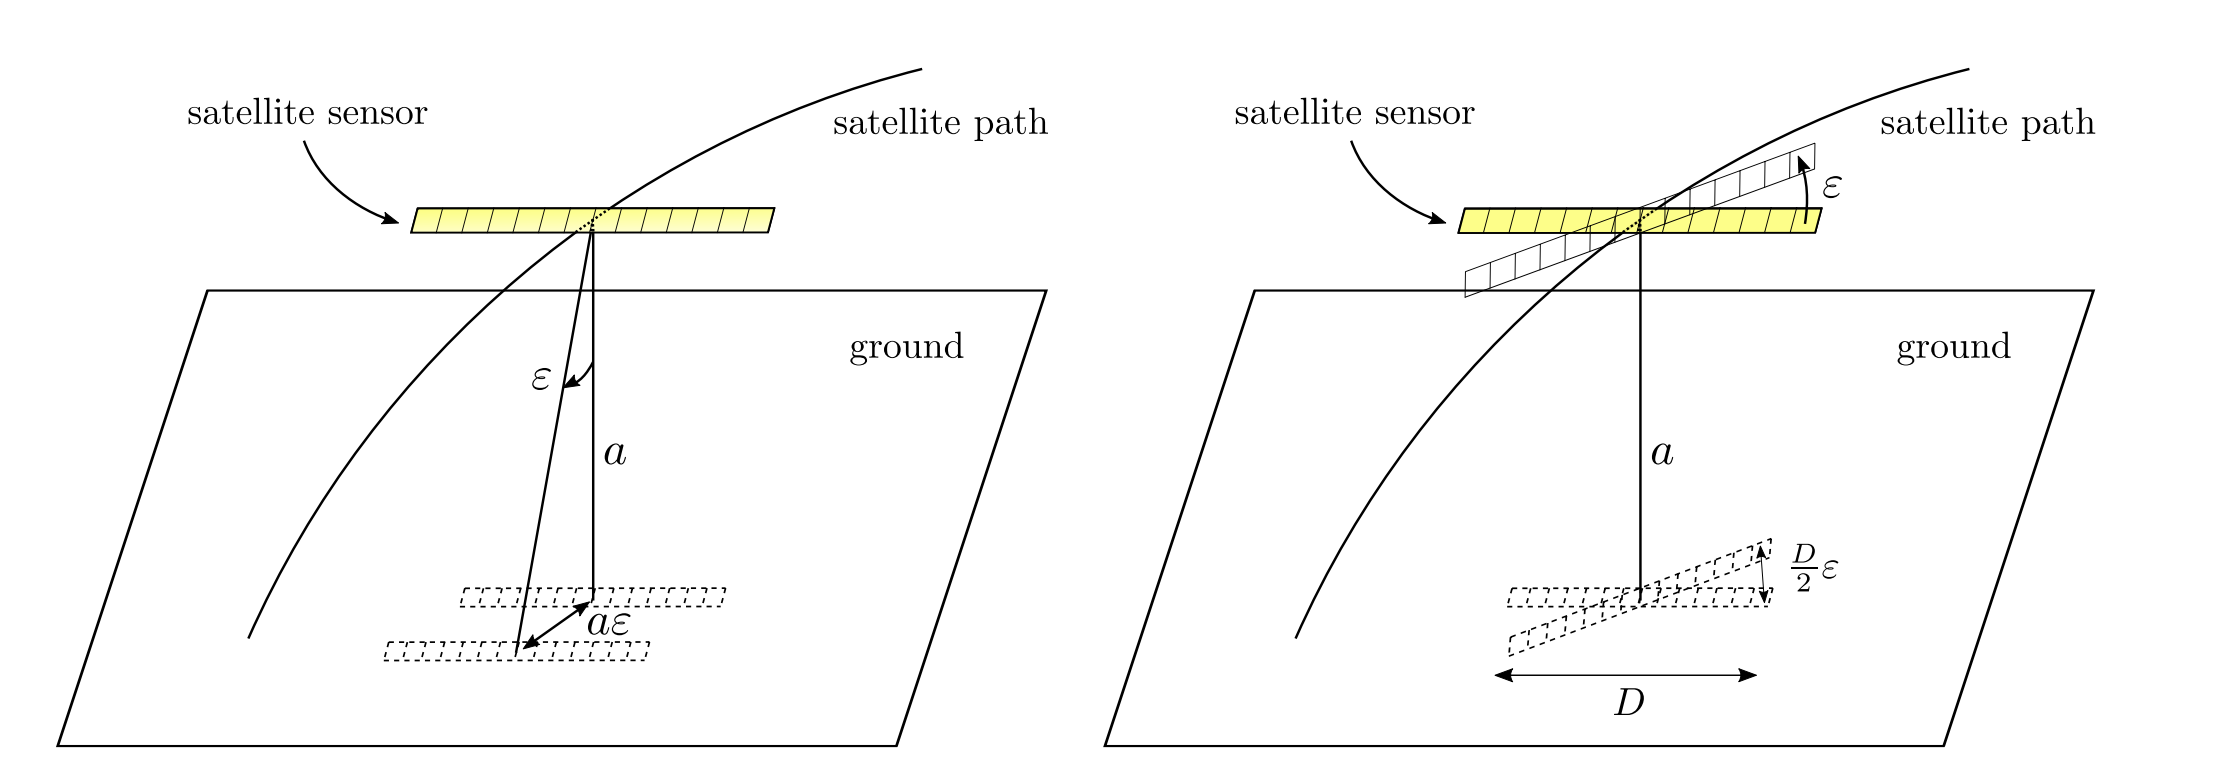
\includegraphics[width=0.8\textwidth]{figures/sensibility.png}
   \caption{Sensibility for roll, pitch and yaw angles.}
   \label{sensiblity}
\end{figure}

For SkySat satellites, if we have an angle error of $\varepsilon \simeq 50 \; \mu \text{rad}$, this leads to an displament of about $0.2 \;\text{m}$  knowing that $D \simeq 9 \;\text{km}$, which corresponds to a distance of about $1$ pixel.
%500 km altitude orbit

\section{Correction of Relative Pointing Error}

A simple and automatic way to correct the pointing error is to transform one of the two images, in such a way that the corresponding points fall on the respective epipolar curves. More formally, given two images $u$, $v$ and a set of correspondences $(\textbf{x}_i , \textbf{x}'_i)_{i=1...N}$ , we search for a transformation $f$ such that, for all $i$, the transformed point $f(\textbf{x}'_i)$ lies on the epipolar curve $\text{epi}^{\textbf{x}_i}_{u v}(R)$.
The desired transformation $f^{*}$ minimises the relative pointing error:
\begin{align}
\label{minif}
f^* = \argmin{f} \dfrac{1}{N} \sum\limits_{i=1}^{N} d(f(\textbf{x}'_i), \text{epi}^{\textbf{x}_i}_{u v}(R))
\end{align}

\subsection{Roll and Pitch Angles}
Because of sensitivity issues, we first can take only roll and pitch error into account. Therefore, according to section \ref{subsec:sensibility}, we search for a transformation $f$ such that
\begin{align*}
f(\textbf{x}) = T\textbf{x}
\end{align*}
where $T$ is a translation:
\begin{align*}
T =
\begin{pmatrix}
1 & 0 & t_x \\
0 & 1 & t_y \\
0 & 0 & 1
\end{pmatrix}
\end{align*}
We can write the transformation $f$, for $ \textbf{x} = (  x \; y \; 1)^T $, as:
\begin{align*}
f(\textbf{x}) = T\textbf{x} =
\begin{pmatrix}
x + t_1 \\
y + t_2 \\
1
\end{pmatrix}
\end{align*}


Without any additional restriction, we may assume that these lines are horizontal (otherwise just do a change of coordinates). This change of coordinates is called \textit{rectification}. We find \\%TODO explain rectification

After rectification, for each point $i$, the horizontal line $F\textbf{x}_i$ can be written as
\begin{align*}
F\textbf{x}_i = \left[ 0 \; 1 \; c_i \right]
\end{align*}
With these notations, for each point correspondence $(\textbf{x}_i , \textbf{x}'_i)$, the pointing error $e$ is:
\begin{align*}
e(\textbf{x}_i, \textbf{x}'_i) = d(\textbf{x}'_i, epi^{\textbf{x}_i}_{u v}(R)) = d(\textbf{x}'_i, F\textbf{x}_i) = | y'_i + c_i|
\end{align*}

Here the error $e$ is invariant to any horizontal translation, thus the search for a translation minimizing the relative pointing error of formula (\ref{minif}) can be restricted to vertical translations only. With a vertical translation of parameter $t$, the global pointing error becomes
\begin{align*}
E = \dfrac{1}{N} \sum\limits_{i=1}^{N} d(T\textbf{x}'_i, F\textbf{x}_i) = \dfrac{1}{N} \sum\limits_{i=1}^{N} | y'_i + t+ c_i|
\end{align*}
The translation that minimizes this sum is given by the geometric median (Weiszfeld, 1937) of the vector $(-y'_i - c_i )_{i=1...N}$.  The pointing error can thus be minimized by applying a translation to one of the images. Note that the median is robust against outliers, thus this correction procedure works well even in the presence of false matches.


\subsection{Roll, Pitch and Yaw Angles}
If we assume that the scene is located at infinity with respect to the satellite, an error in the sensor attitude measurement can be modeled in image space as a translation composed with a rotation. Therefore we have
\begin{align*}
f(\textbf{x}) = TR\textbf{x}
\end{align*}
where $R$ is a rotation and $T$ a translation:\\
\begin{align*}
R =
\begin{pmatrix}
\cos(\theta) & -\sin(\theta) & 0 \\
\sin(\theta) & \cos(\theta) & 0 \\
0 & 0 & 1
\end{pmatrix}, \;
T =
\begin{pmatrix}
1 & 0 & t_x \\
0 & 1 & t_y \\
0 & 0 & 1
\end{pmatrix}
\end{align*}

\subsubsection{Approximation of the Rotation}

To correct the pointing error in the rectified setting we find $R^*$ and $T^*$ minimizing the pointing error defined as follow :
\begin{align}
    (R^*, T^*) = \argmin{R,T} \sum_{i=1}^N d(TR\bm{x_i'}, F\bm{x}_i)^2
\end{align}
As in~\cite{de2014b}

After rectification, the horizontal line $F\bm{x}_i$ can be written, in homogeneous coordinates, as
\begin{align*}
F\bm{x}_i =  \begin{bmatrix} 0 & 1 & y_i \end{bmatrix}
\end{align*}
With these notations, if the model now includes a rotation $R$, for each point correspondence $(\bm{x}_i , \bm{x}'_i)$, we have
\begin{align*}
e(\textbf{x}_i, \textbf{x}'_i) = d(TR\bm{x}'_i, \text{epi}^{\bm{x}_i}_{u v}(R)) = d(TR\bm{x}'_i, F\bm{x}_i) = |x_i' \sin \theta   + y_i' \cos \theta  + t - y_i |
\end{align*}
where $\theta$ is the angle of the rotation.

We can consider that $\theta$ is small enough compare to $2\pi$. In fact on satellites such as Sentinel or Pleiades (%TODO source)
the precision of the yaw angle is around $50~\mu \text{rad}$. Even if Planet's sensor would be $100$ less precise, we will still have an yaw angle less than $1$ degree.
With this approximation, we can write:
\begin{align*}
e(\textbf{x}_i, \textbf{x}'_i) = |x_i' \theta   + y_i' + t - y_i |
\end{align*}

Correcting the global pointing error is to minimize:
\begin{align*}
(\theta^*, t^*) = \argmin{\theta,t} \sum_{i=1}^N d(TR\bm{x_i'}, F\bm{x}_i)^2 = \sum_{i=1}^N (x_i' \theta   + y_i' + t - y_i)^2
\end{align*}
We can write this optimization problem as :
\begin{align*}
X^* = \argmin{X} \| AX + b \|^2
\end{align*}
where
\begin{align*}
A =
\begin{pmatrix}
x_1' & 1 \\
x_2' & 1 \\
\vdots & \vdots \\
x_n' & 1 \\
\end{pmatrix} \quad
X =
\begin{pmatrix}
\theta \\
t
\end{pmatrix} \quad
b =
\begin{pmatrix}
y_1' - y_1\\
y_2' - y_2\\
\vdots\\
y_1' - y_1\\
\end{pmatrix}
\end{align*}

The solution of this optimization problem is the solution of the normal equation
\begin{align*}
 A^TAX = -A^Tb
\end{align*}
Here,
\begin{align*}
A^TA =
\begin{pmatrix}
\sum\limits_{i=1}^N x_{i}'^2 & \sum\limits_{i=1}^Nx_{i}' \\
\sum\limits_{i=1}^N x_{i}' & N \\
\end{pmatrix}
\end{align*}
So $A^TA$ is inversible, and the optimal correction in the rectified images is:
\begin{align*}
\begin{pmatrix}
\theta^* \\
t^*
\end{pmatrix} = X^* = -(A^TA)^{-1}A^Tb
\end{align*}


\subsubsection{Solving Numerically an Optimization Problem}
To correct the pointing error in the rectified setting we find $R^*$ and $T^*$ minimizing the pointing error defined as follow :
\begin{align}
    (R^*, T^*) = \argmin{R,T} \sum_{i=1}^N d(RT\bm{x_i'}, F\bm{x}_i)
\end{align}

Since we are not able to solve this optimization problem analytically, we solve it numerically thanks to the L-BFGS algorithm. As input are the correspondences on the images and the affine approximation matrix and the optimization algorithm outputs the optimal angle $\theta \in [0, 2\pi]$ corresponding to the error on the yaw and a translation $t \in \mathbb{R}$ corresponding to a translation in the normal direction w.r.t. the epipolar lines.

\paragraph*{Limited-memory BFGS\\}
Limited-memory BFGS is an optimization algorithm in the family of quasi-Newton methods that approximates the BFGS algorithm using a limited amount of computer memory. In our case we do not need to compute the gradient analytically since the algorithm approximates it using finite difference. We use this algorithm as a black box to solve the minimization problem.

\newpage
\section{Data overview}

\subsection{Test data}

S2P pipeline comes with a pair and a triplet of test data captured by Pleiades. The input pair and their geolocalisation is shown below in Figure~\ref{fig_geoloc_testdata}. After the pair, the triplet is also represented in Figure~\ref{fig_geoloc_testdata_triplet}. The expected output result is also shown in Figure~\ref{fig_expected_output_pair} for the pair, and is offline visuable using the PotreeConverter module available on github~\cite{PotreeConverter}.

\begin{figure}[H]
    \centering
    \begin{subfigure}[t]{0.8\textwidth}
        \centering
        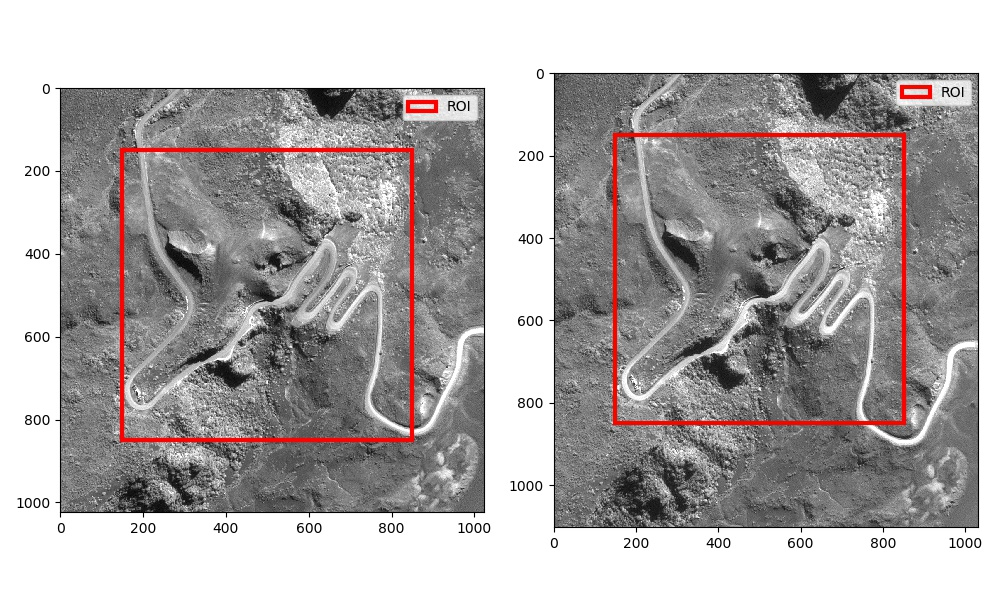
\includegraphics[width = 0.95\textwidth]{ROI_testdata_pair.jpeg}
        \caption{Region of intereset (ROI, in red) in test data input pair}
    \end{subfigure}%
    ~
    \vfill
    ~
    \begin{subfigure}[t]{0.8\textwidth}
        \centering
        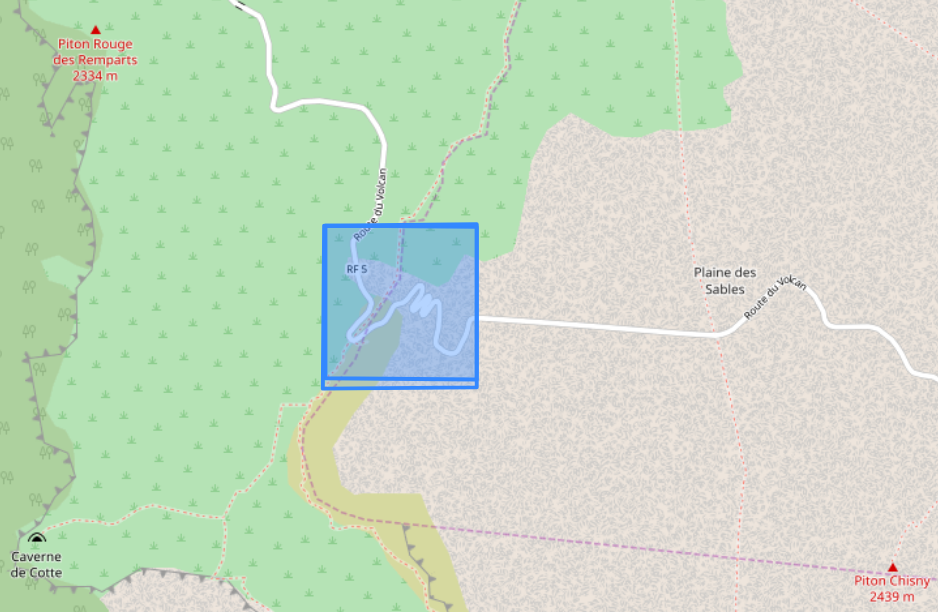
\includegraphics[width = 0.95\textwidth]{geoloc_testdata.png}
        \caption{Geolocalisation of the test data input pair, in La Réunion. Reprojected using an elevation of $h=2350~m$. Center of ROI $(lat, lon) ~\approx (-21.23066754, 55.65022517)$}
    \end{subfigure}%
    \caption{Overview of the test data input pair}
    \label{fig_geoloc_testdata}
\end{figure}

\begin{figure}[H]
    \centering
    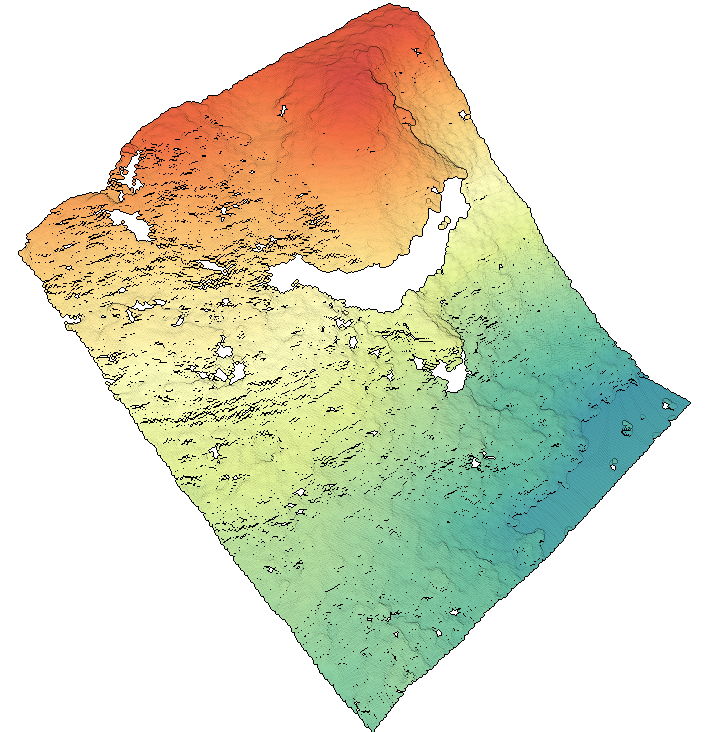
\includegraphics[height = 0.4\textheight]{elevation_intro.png}
    \caption{Expected output from PotreeConverter~\cite{PotreeConverter} of S2P on test data input pair.}
    \label{fig_expected_output_pair}
\end{figure}



\begin{figure}[H]
    \centering
    \begin{subfigure}[t]{0.8\textwidth}
        \centering
        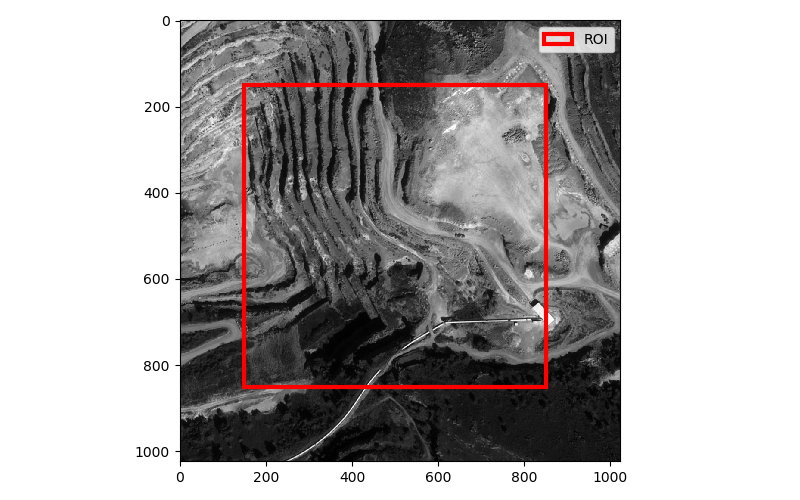
\includegraphics[width = 0.95\textwidth]{ROI_testdata_triplets.png}
        \caption{Region of intereset (ROI, in red) in test data input triplet. Only one (img\_01.tif) of the 3 images is represented.}
    \end{subfigure}%
    ~
    \vfill
    ~
    \begin{subfigure}[t]{0.8\textwidth}
        \centering
        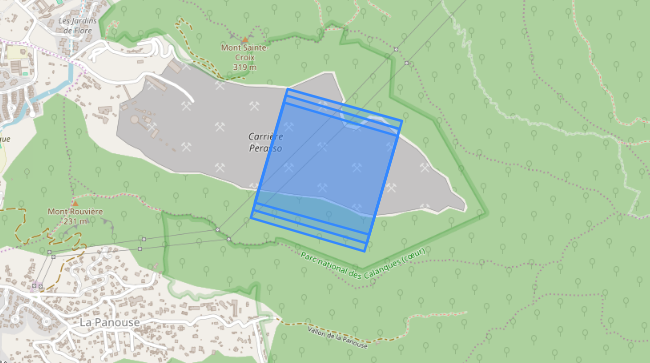
\includegraphics[width = 0.95\textwidth]{geoloc_testdata_triplets.png}
        \caption{Geolocalisation of the test data input triplet, east of Marseille. Reprojected using an elevation of $h=300~m$. Center of ROI $(lat, lon) ~\approx (43.26182762, 5.443071)$}
    \end{subfigure}%
    \caption{Overview of the test data input triplet}
    \label{fig_geoloc_testdata_triplet}
\end{figure}

\subsection{Planet Data}

Data provided are coming from Skysat-2 and Skysat-3 which are made of 3 camera each, with a revisit time of $3$ to $4$ day at $500~km$ altitude~\cite{planet_product}. The agility of Skysat satellite is 2.3 target (6.6 x 10 km) per minute. The resolution of the panchromatic images is $0.9~m$, and academics can apply to their Education and Research program to download up to $10000~\text{km}^2/\text{month}$ of those data.

\subsubsection{Structure}

The structure of the provided Skysat-2 data are represented in figure~\ref{fig_forest_skysat_2}. Each trace is identified with a catalog ID, for example s03\_20161003T161107Z, which uniquely identifies the trace for s03 (Skysat-3) timed at $16:11:07$ Zoulou the $03/10/2016$. For each trace, the panchromatic and the pansharp data are available; nonetheless, we only used the panchromatic ones. The 3 detectors of skysat are then identified with $d1$, $d2$ and $d3$, and images from each detector captured during the trace are stored as a trip of single frames, with a small horizontal and vertical overlap. With each tif image file comes the rpc model stored in ikonos convention. Each image is numbered between $1$ and $18$ for each detector, and the common POSIX time for a number for the three detectors is stored in the RPC file associated with the take. For the 3 detectors, the necessary time to capture the 18 images is approximately $9.2~s$. The mosaic of data is available in appendix~\ref{appen_mosaic}.

The structure of the provided Skysat-3 data are simpler: 892 panchromatic frames were collected from $02:05:54$ Zoulou to $02:06:23$ Zoulou the $07/05/2015$.

\begin{figure}[H]
    \centering
    \resizebox{!}{.7\textheight}{
    \begin{forest}
      my label/.style={
        label={[font=\sffamily]right:{#1}},
      },
      for tree={
        folder,
        font=\sffamily,
        text=white,
        minimum height=0.75cm,
        if level=0{fill=ForestGreen}{fill/.wrap pgfmath arg={SlateBlue#1}{int(4-(mod((level()-1),4)))}},
        rounded corners=4pt,
        grow'=0,
        edge={ForestGreen,rounded corners,line width=1pt},
        fit=band,
      },
      [data
        [s03\_20161003T161107Z
          [panchromatic
            [s03\_20161003T161107Z\_pan\_d1\_0001\_rpc.txt]
            [s03\_20161003T161107Z\_pan\_d1\_0001.tif]
          ]
          [pansharp
            [s03\_20161003T161107Z\_pansharp\_bgrn\_d1\_0001\_rpc.txt]
            [s03\_20161003T161107Z\_pansharp\_bgrn\_d1\_0001.tif]
          ]
        ]
        [s03\_20161003T161148Z
          [panchromatic
            [s03\_20161003T161148Z\_pan\_d1\_0001\_rpc.txt]
            [s03\_20161003T161148Z\_pan\_d1\_0001.tif]
          ]
          [pansharp
            [s03\_20161003T161148Z\_pansharp\_bgrn\_d1\_0001\_rpc.txt]
            [s03\_20161003T161148Z\_pansharp\_bgrn\_d1\_0001.tif]
          ]
        ]
        [s03\_20161003T161231Z
          [panchromatic
            [s03\_20161003T161231Z\_pan\_d1\_000\_rpc.txt]
            [s03\_20161003T161231Z\_pan\_d1\_0001.tif]
          ]
          [pansharp
            [s03\_20161003T161231Z\_pansharp\_bgrn\_d1\_0001\_rpc.txt]
            [s03\_20161003T161231Z\_pansharp\_bgrn\_d1\_0001.tif]
          ]
        ]
      ]
  \end{forest}
  }

    \caption{Structure of the provided Skysat-2 data}
    \label{fig_forest_skysat_2}
\end{figure}

\subsubsection{Geolocalisation}

The geolocalisation have been done using the rpc model, with a reprojection altitude depending of the area considered: for Skysat-2, near Cushing (United States), an altitude of $h=285~m$ (mean altitude of Cushing) has been used, while an altitude of $h=0m$ has been used for Skysat-3 video, in port Hedland (Australia). The three traces for Skysat-2 are shown in chronological order in figures~\ref{fig_trace_7Z}~\ref{fig_trace_8Z}~\ref{fig_trace_1Z}, while the trace for Skysat-3 only represents the 1t, 300th, and 600th images in the video. All the geographic content are brought to us thanks to OpenStreeMap API~\cite{OpenStreetMap}.


\begin{figure}[H]
    \centering
    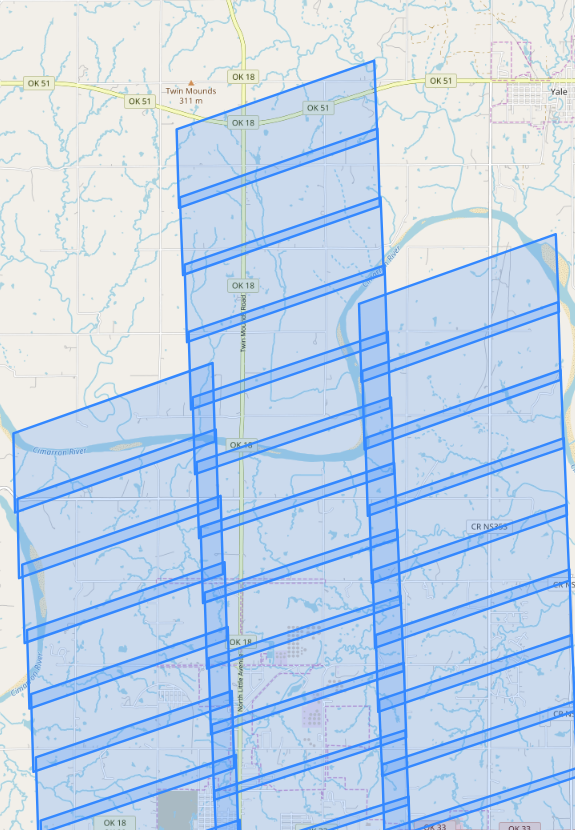
\includegraphics[height = 0.7\textheight]{trace_7Z.png}
    \caption{Geolocalisation of trace s03\_20161003T161107Z near Cushing (United States). Reprojected using an elevation of $h=285~m$}
    \label{fig_trace_7Z}
\end{figure}

\begin{figure}[H]
    \centering
    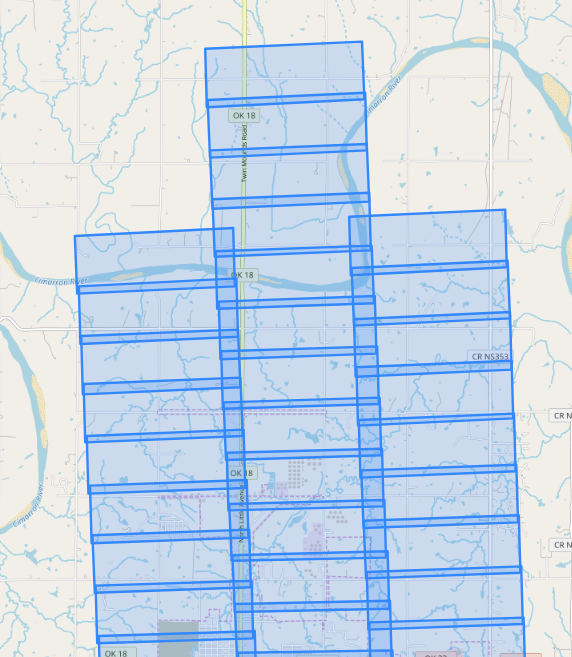
\includegraphics[height = 0.7\textheight]{trace_8Z.png}
    \caption{Geolocalisation of trace s03\_20161003T161148Z near Cushing (United States). Reprojected using an elevation of $h=285~m$}
    \label{fig_trace_8Z}
\end{figure}

\begin{figure}[H]
    \centering
    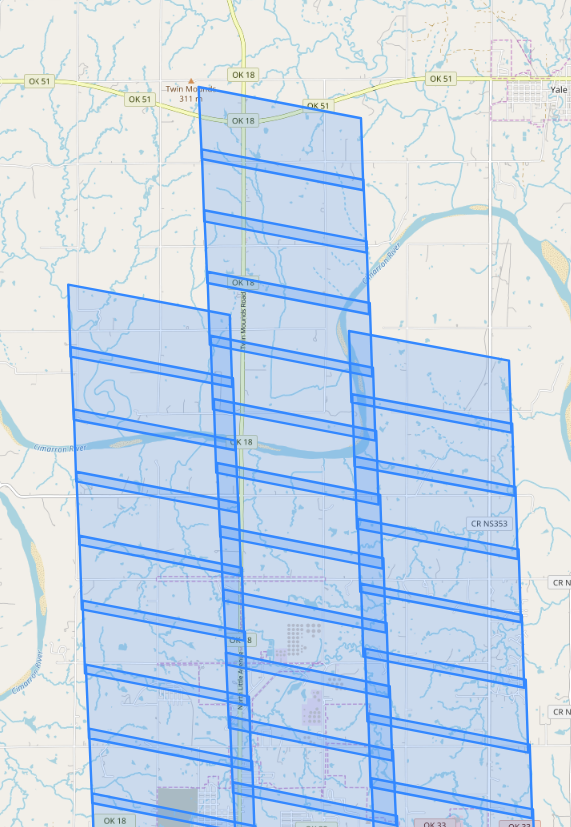
\includegraphics[height = 0.7\textheight]{trace_1Z.png}
    \caption{Geolocalisation of trace s03\_20161003T161231Z near Cushing (United States). Reprojected using an elevation of $h=285~m$}
    \label{fig_trace_1Z}
\end{figure}

\begin{figure}[H]
    \centering
    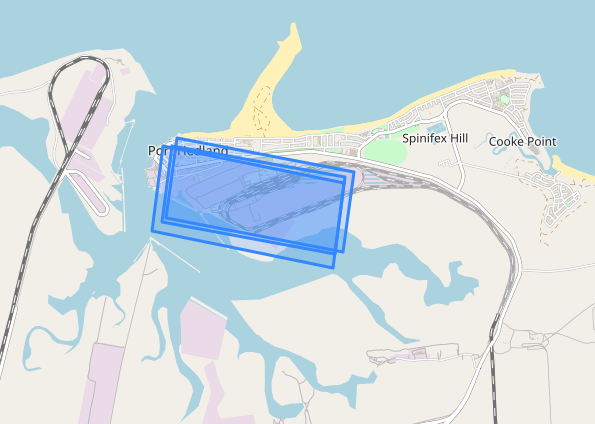
\includegraphics[width = 0.8\textwidth]{trace_video.png}
    \caption{Geolocalisation of trace s02\_20150507T020554Z in Port Hedland (Australia). Reprojected using an elevation of $h=285~m$}
    \label{fig_trace_video}
\end{figure}

\newpage
\section{Experimental Results}

 \subsection{Error evolution}

 We experiment with different ways of correcting the pointing error.
 \begin{enumerate}
 \item Translation: analytically without rectification
 \item Translation: numerically with rectification (one degree of freedom for the translation)
  \item Translation: numerically without rectification (two degrees of freedom for the translation)
   \item Translation and rotation: numerically with rectification (one degree of freedom for the translation)
    \item Translation and rotation: numerically without rectification (two degrees of freedom for the translation)
 \end{enumerate}
Unfortunately, we did not test the analytical way of correcting the pointing error with translation and rotation due to the time constraint of the project and code issues.

 \subsubsection{Testdata (Pléiades)}
 We first try our modified pipeline with improved pointing error correction on Pléiades images (see Figure \ref{fig:testdata}) from the \verb|s2p| Github repository. These images are located on the island of Reunion. We can observe on Figure \ref{fig_geoloc_testdata} the error of the RPC function of the two images.\\

            \begin{figure}[H]
            \centering
            \begin{subfigure}[b]{0.5\linewidth}
              \centering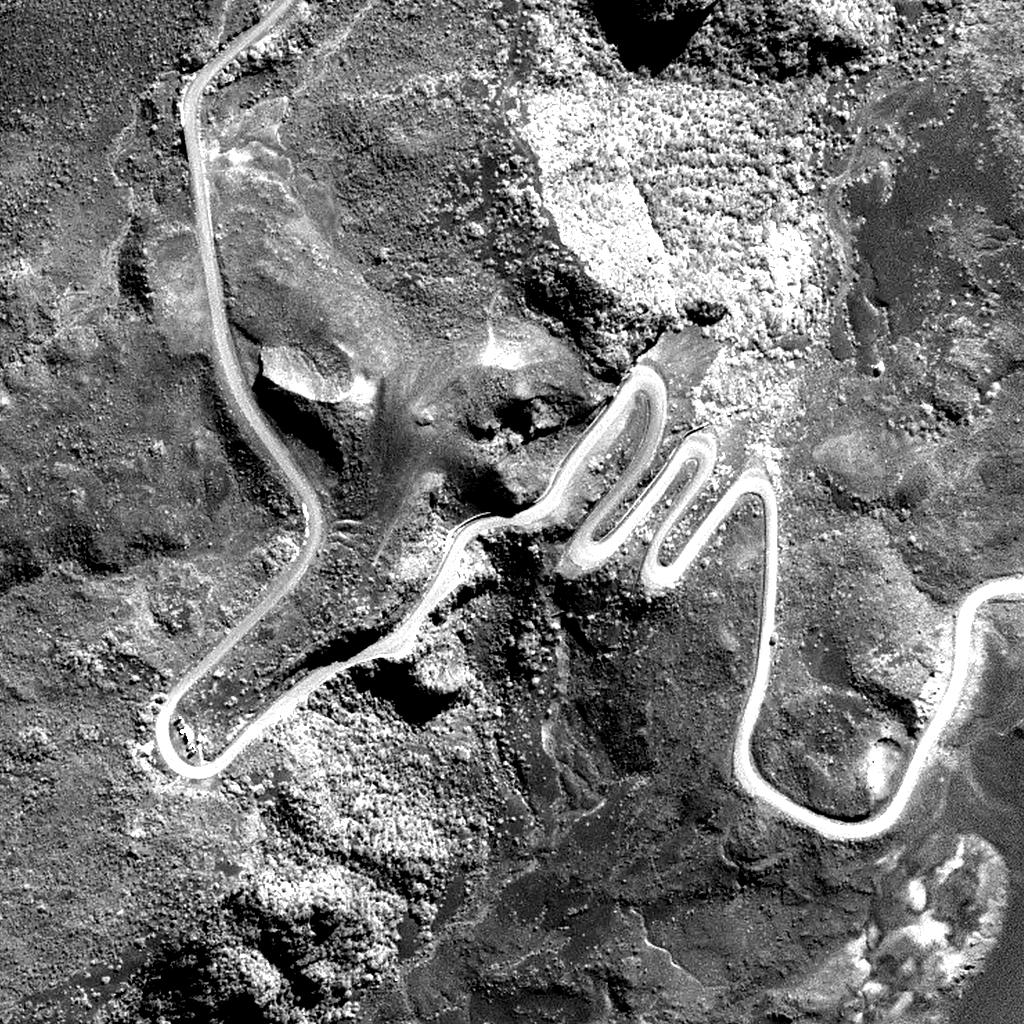
\includegraphics[width=0.95\textwidth]{figures/testdata_1.jpeg}
            \end{subfigure}%
            \begin{subfigure}[b]{0.5\linewidth}
              \centering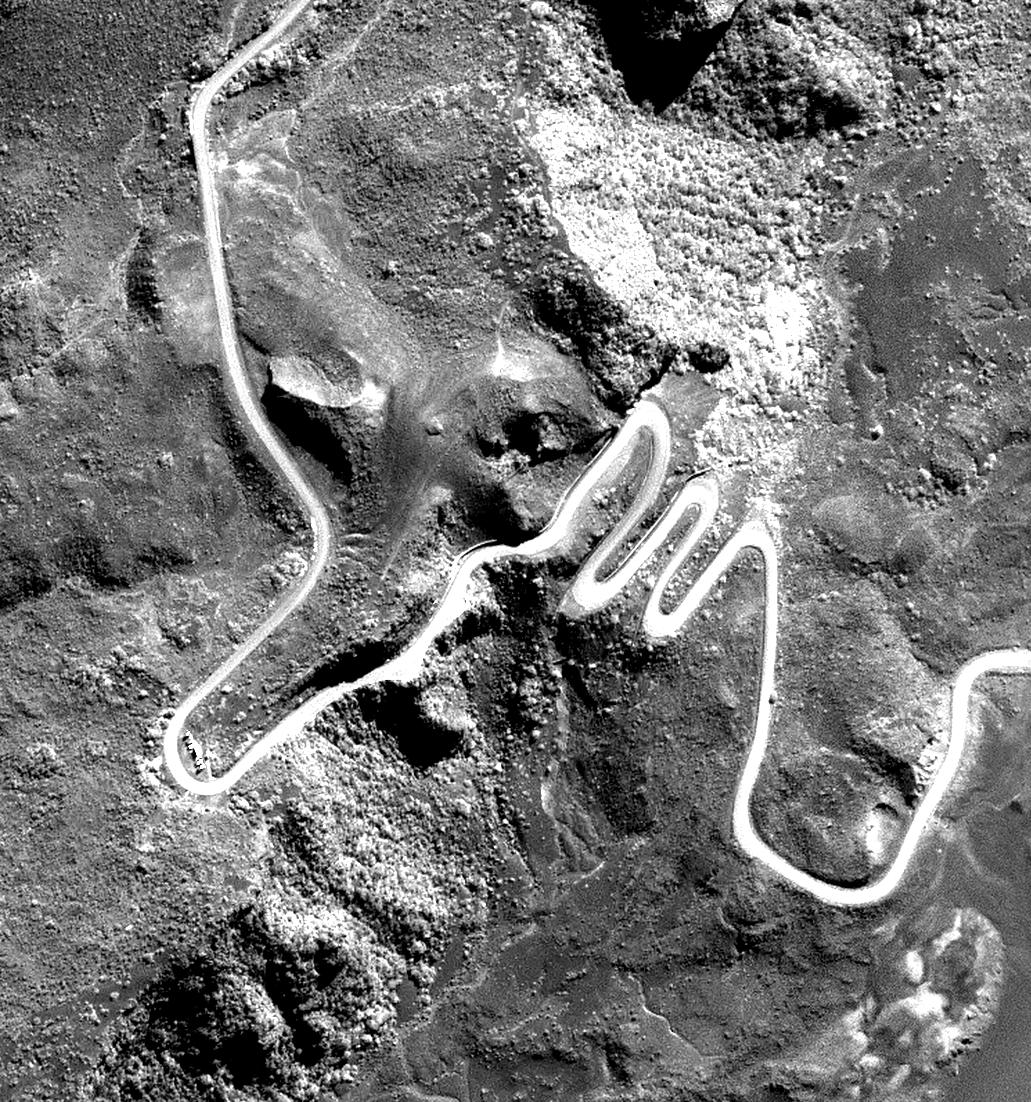
\includegraphics[width=0.9\textwidth]{figures/testdata_2.jpeg}
            \end{subfigure}
            \caption{Pléiades images of the Réunion}
             \label{fig:testdata}
          \end{figure}

 Results from the different methods are compiled in Table \ref{tab:testdata-res}. The images were divided into $9$ tiles of $300 \times 300$ pixels.

\begin{table}[h]
\centering
             \begin{tabular}{|r||c|c|c|c|c|c|c|c|c|}
              \hline
           methods &   tile 1 & tile 2 & tile 3 & tile 4 & tile 5 & tile 6 & tile 7 & tile 8 & tile 9\\
              \hline
          no correction &   63.1& 239.5& 266.1& 130.9& 243.6& 165.1& 84.2& 152.7& 150.5 \\
             \hline
      (1) &  19.4& 48.2& 51.8& 45.0& 55.4& 28.2& 22.8& 37.6& 35.8\\
       (2) & 19.4& 48.2& 51.8& 45.0& 55.4& 28.2& 22.8& 37.6& 35.8\\
       (3) & 19.4& 48.2& 51.8& 45.0& 55.4& 28.2& 22.8& 37.6& 35.8\\
      (4) & 19.9& 47.4& 55.3& 43.5& 54.6& 28.2& 27.8& 34.9& 42.3\\
      (5)  & 19.4& 47.4& 55.3& 43.5& 54.6& 28.2& 27.8& 33.6& 42.3\\
              \hline
            \end{tabular}
            \caption{Results of pointing error correction on Pléiades images}
             \label{tab:testdata-res}
          \end{table}


 \subsubsection{Vidéo SkySat}
             We then try our modified pipeline with improved pointing error correction on two images from the Skysat videos (see Figure \ref{fig:video}) from Planet's data. The video were shot on an harbor in Australia. We can see on Figure \ref{fig_trace_video} the error of the RPC function of all the images of the video.\\

            \begin{figure}[H]
            \centering
            \begin{subfigure}[b]{0.8\linewidth}
              \centering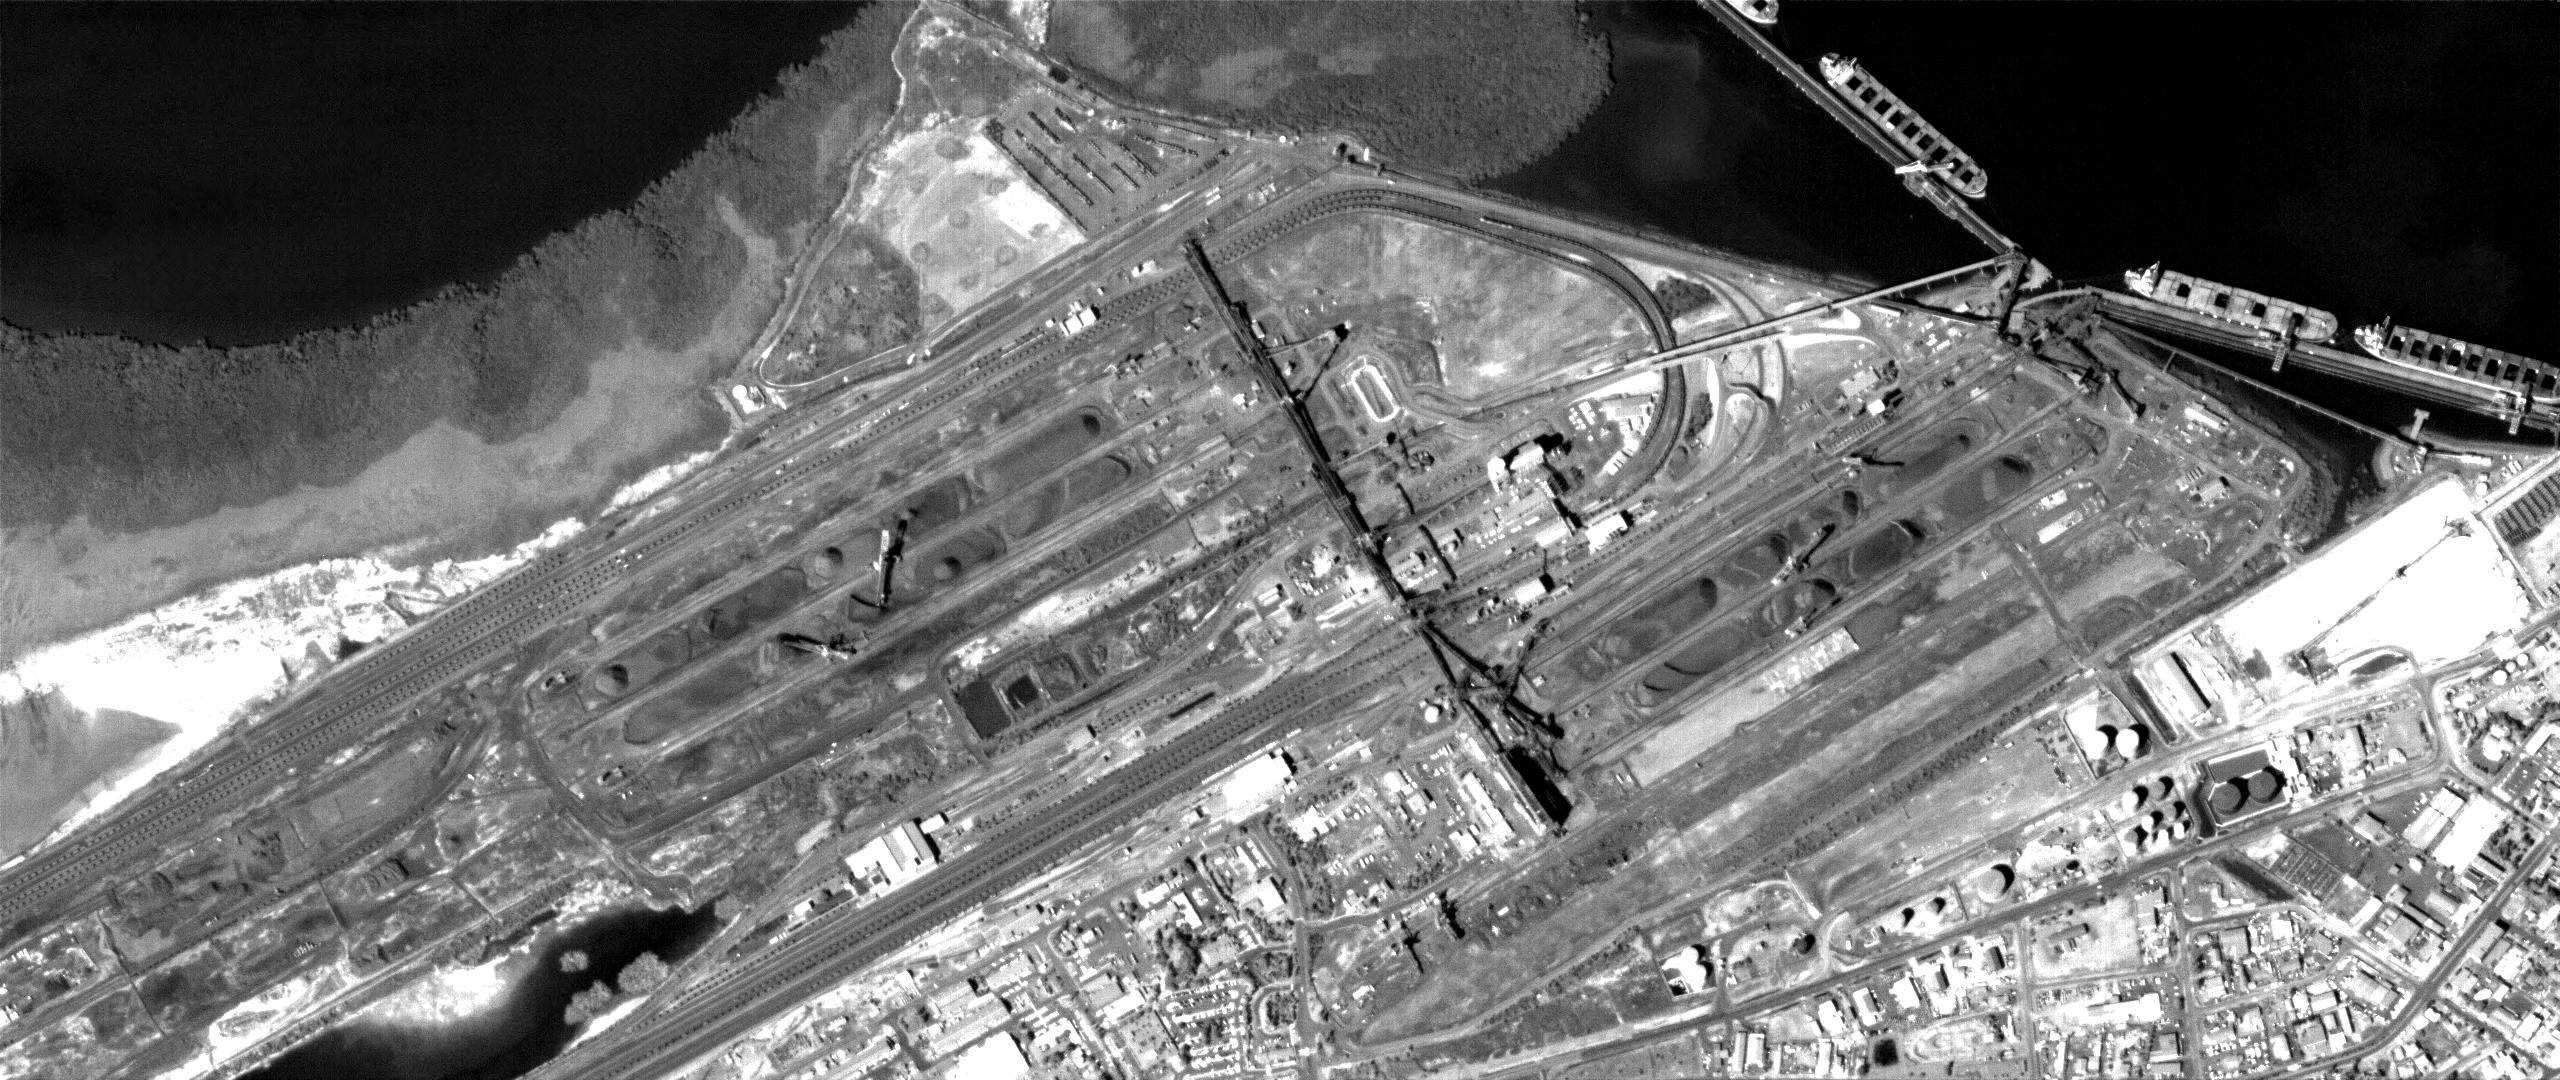
\includegraphics[width=\textwidth]{figures/video_1.jpeg}
            \end{subfigure}%

            \begin{subfigure}[b]{0.8\linewidth}
              \centering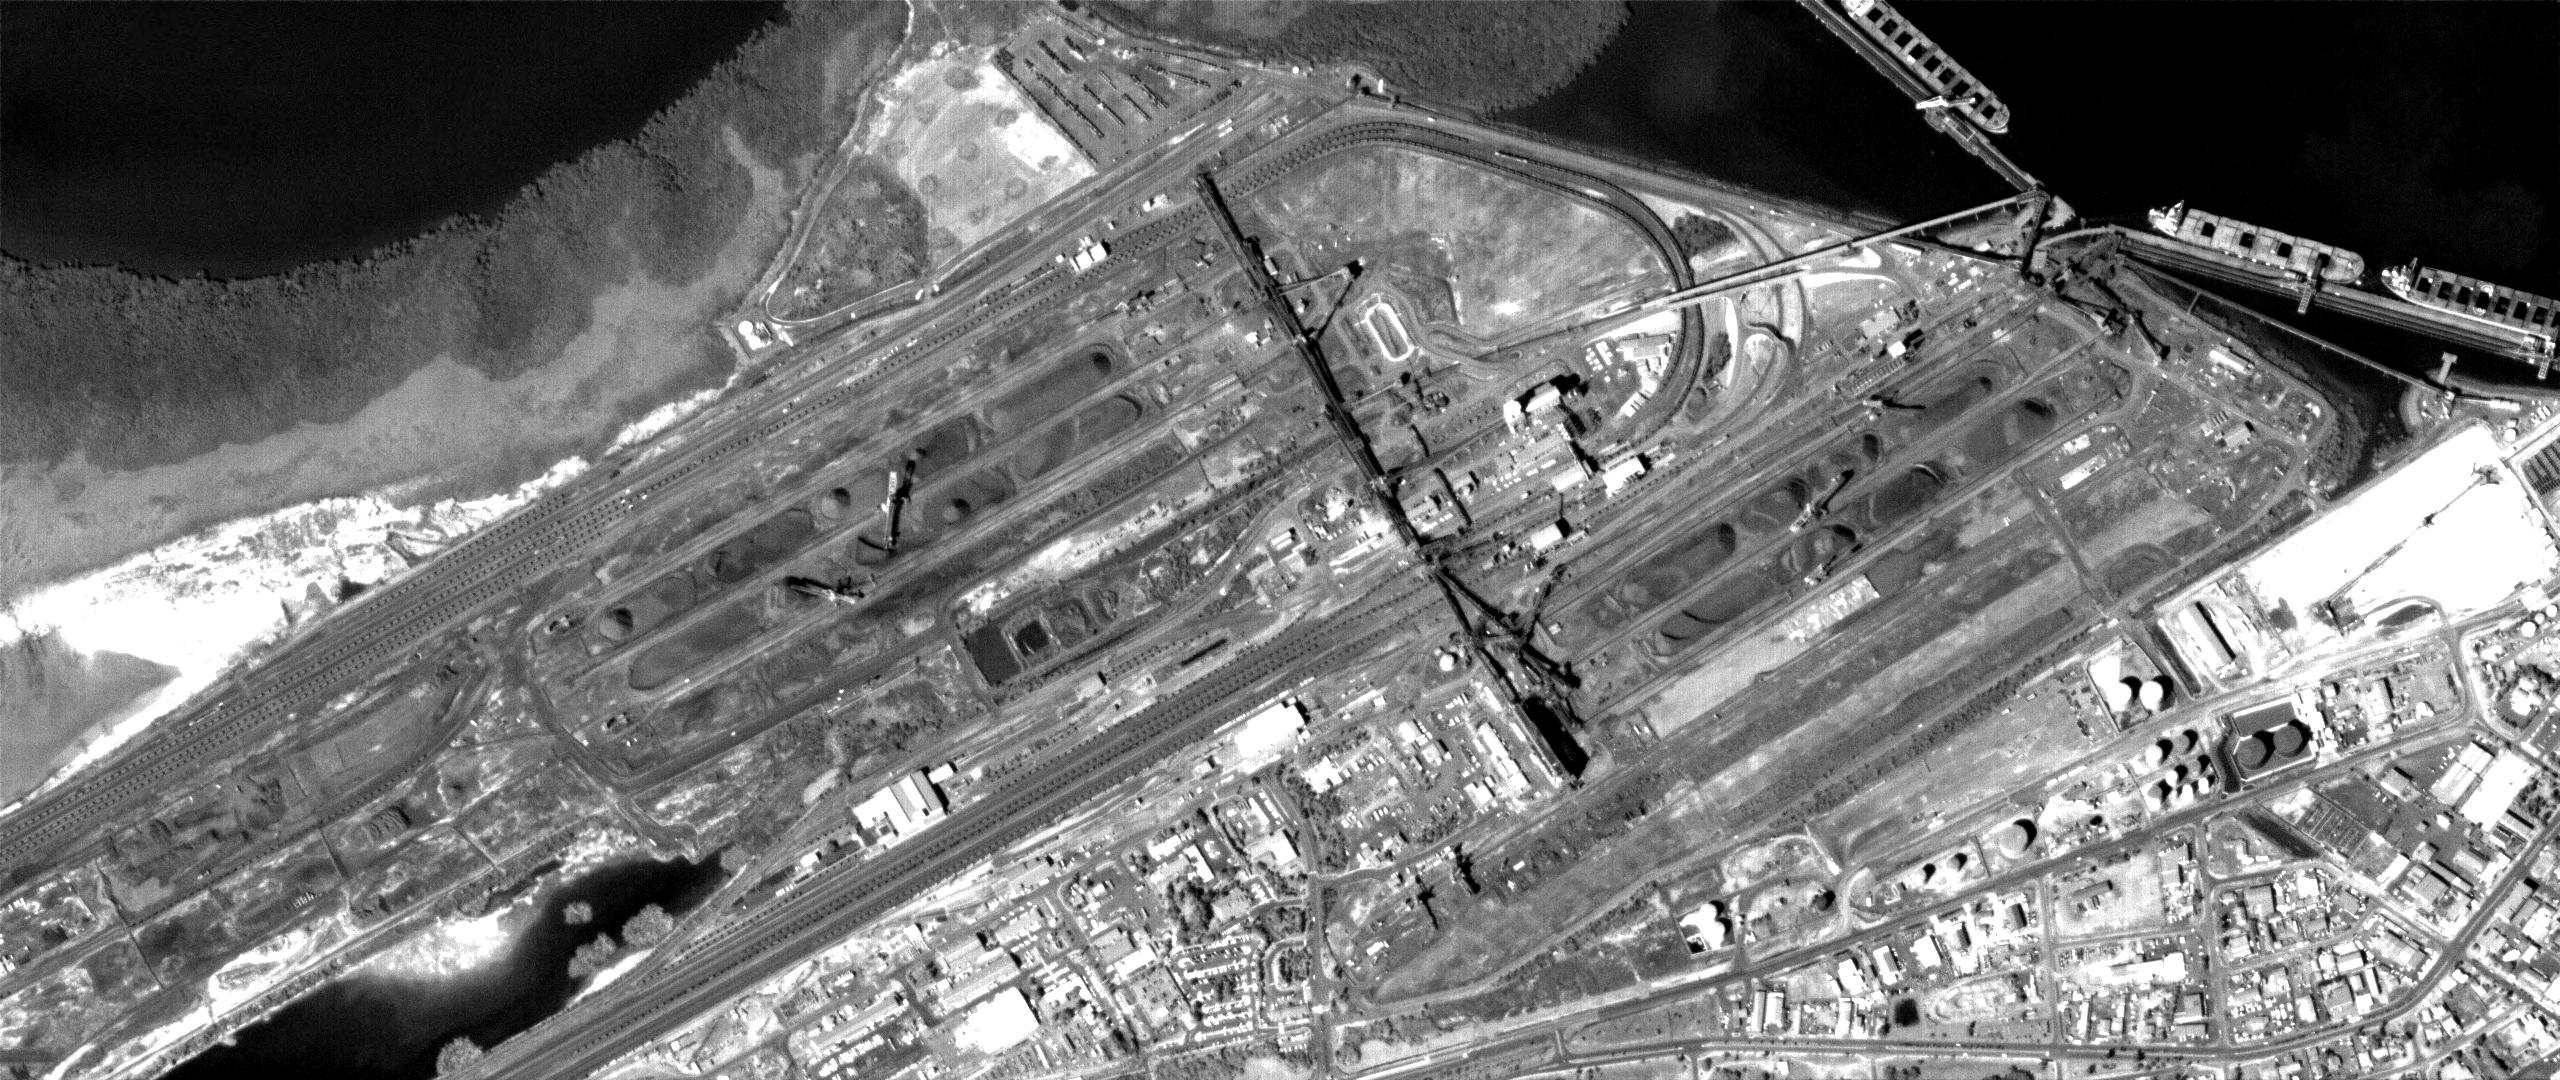
\includegraphics[width=\textwidth]{figures/video_100.jpeg}
            \end{subfigure}
           \caption{First and $100$-th images of a SkySat video.}
           \label{fig:video}
          \end{figure}


Results from the different methods are compiled in Table \ref{tab:video-res}. The images were divided into $3$ tiles of $1000 \times 1000$ pixels.

\begin{table}[h]
\centering
             \begin{tabular}{|r||c|c|c|}
              \hline
            methods &     tile 1 & tile 2 & tile 3 \\
              \hline
          no correction &   50.4& 36.6& 91.8 \\
             \hline
      (1) & 47.7& 32.8& 54.6\\
     (2) & 47.7& 32.8& 54.6\\
      (3) & 47.7& 32.8& 54.6\\
      (4) & 49.7& 29.1& 70.7\\
      (5) & 42.6& 29.1& 70.7\\
              \hline
            \end{tabular}
                 \caption{Results of pointing error correction on images from the Skysat's video.}
             \label{tab:video-res}
          \end{table}

\subsubsection{Triplet SkySat}
             We then try our modified pipeline with improved pointing error correction on two images from the Skysat triplets (see Figure \ref{fig:triplet}) from Planet's data. The images are taken in the USA. %We can see on Figure \ref{fig:video-location} the error of the RPC function of all the images of the video.\\

            \begin{figure}[H]
            \centering
            \begin{subfigure}[b]{0.6\linewidth}
              \centering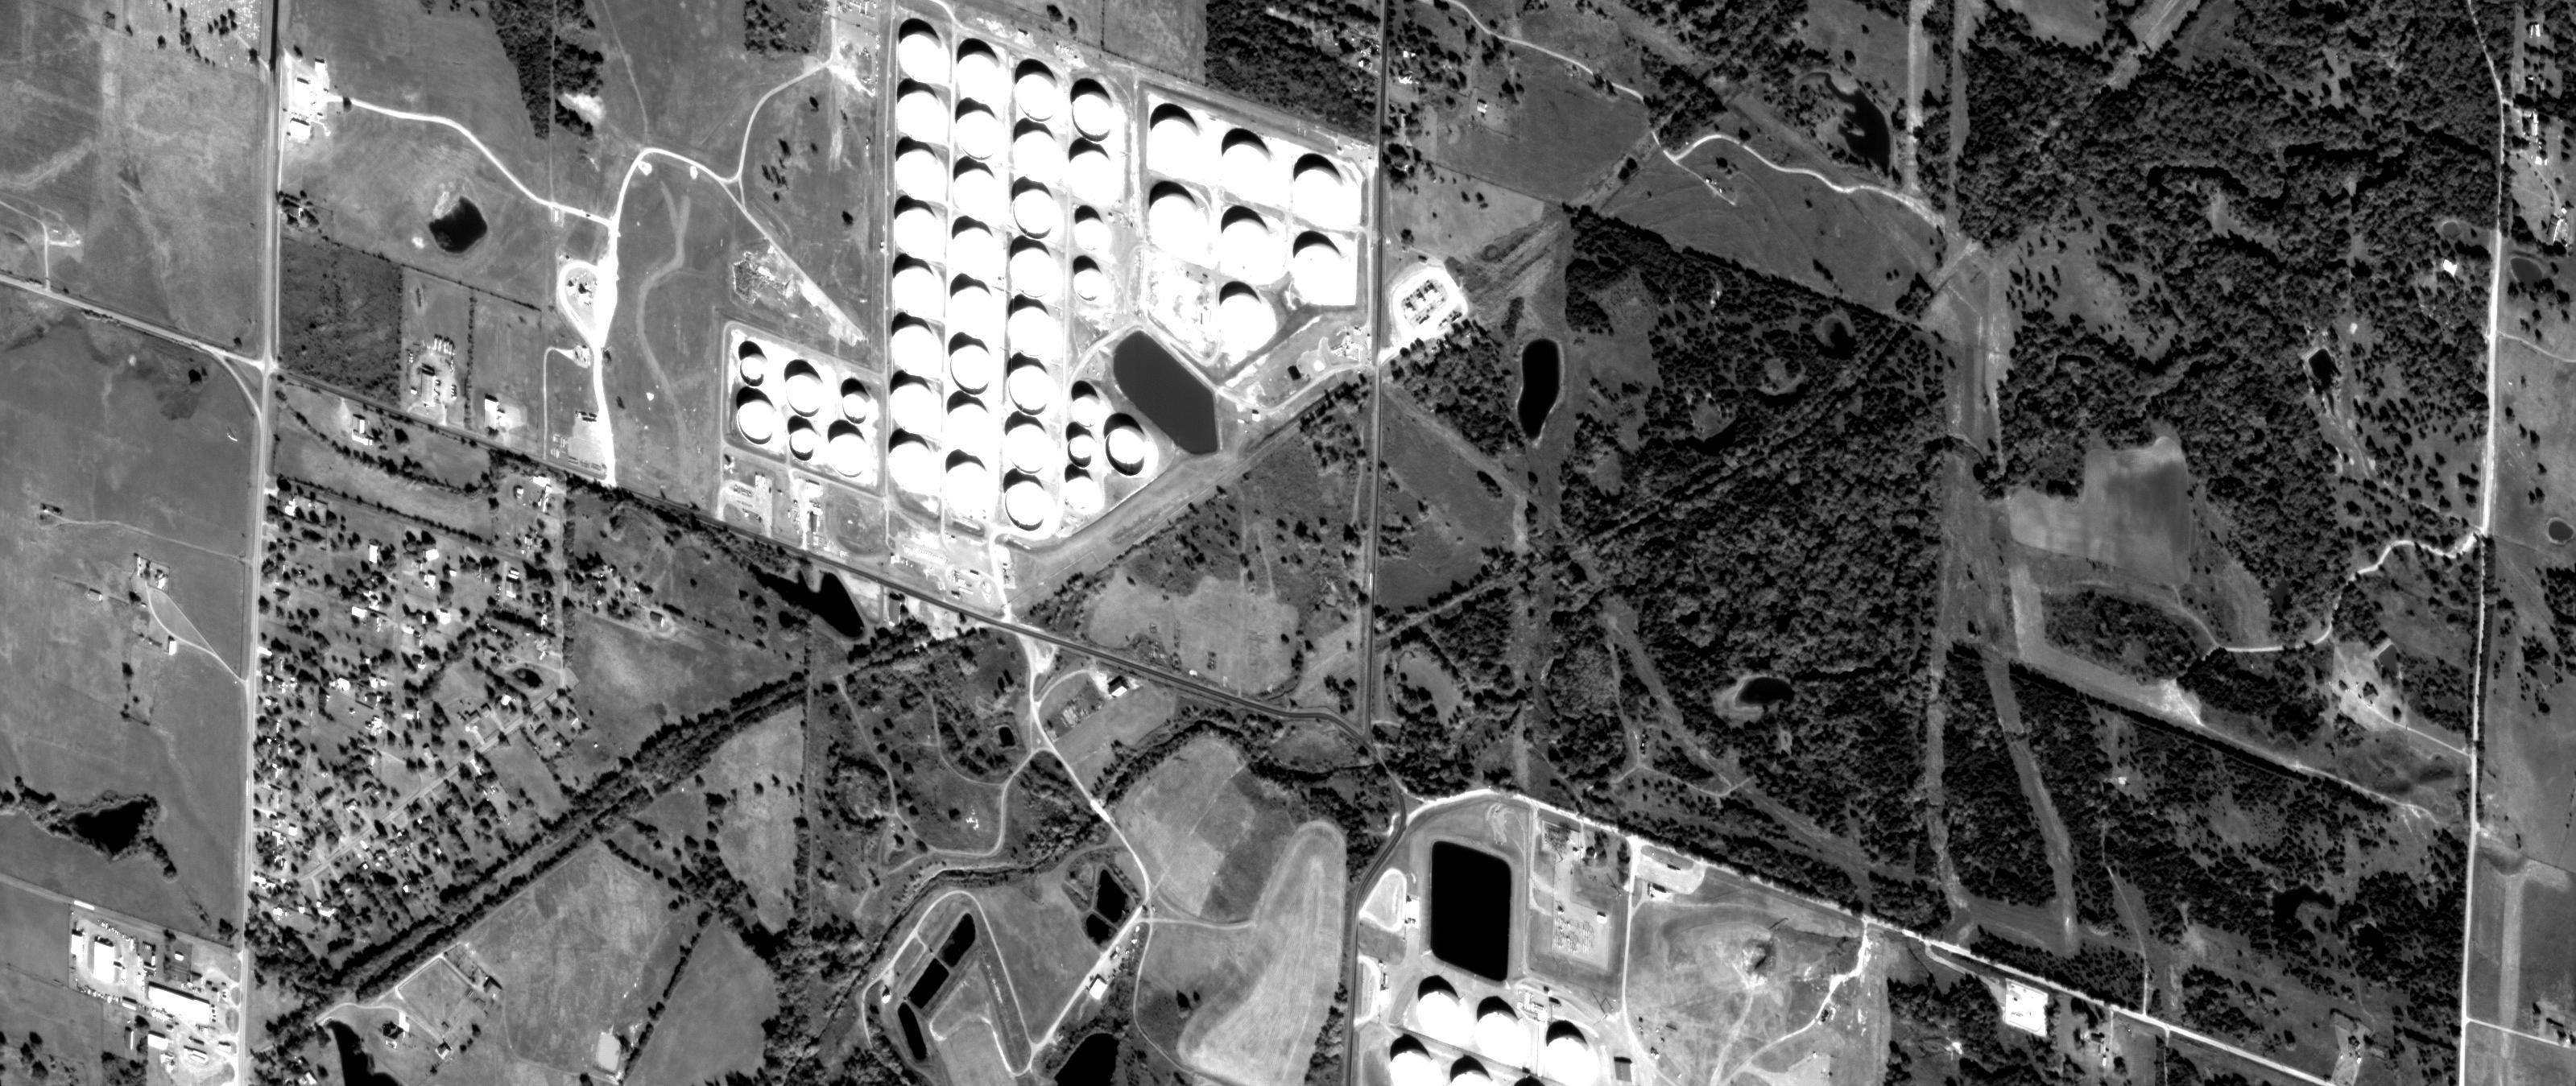
\includegraphics[width=0.9\textwidth]{figures/triplet_0.jpeg}
            \end{subfigure}%

            \begin{subfigure}[b]{0.6\linewidth}
              \centering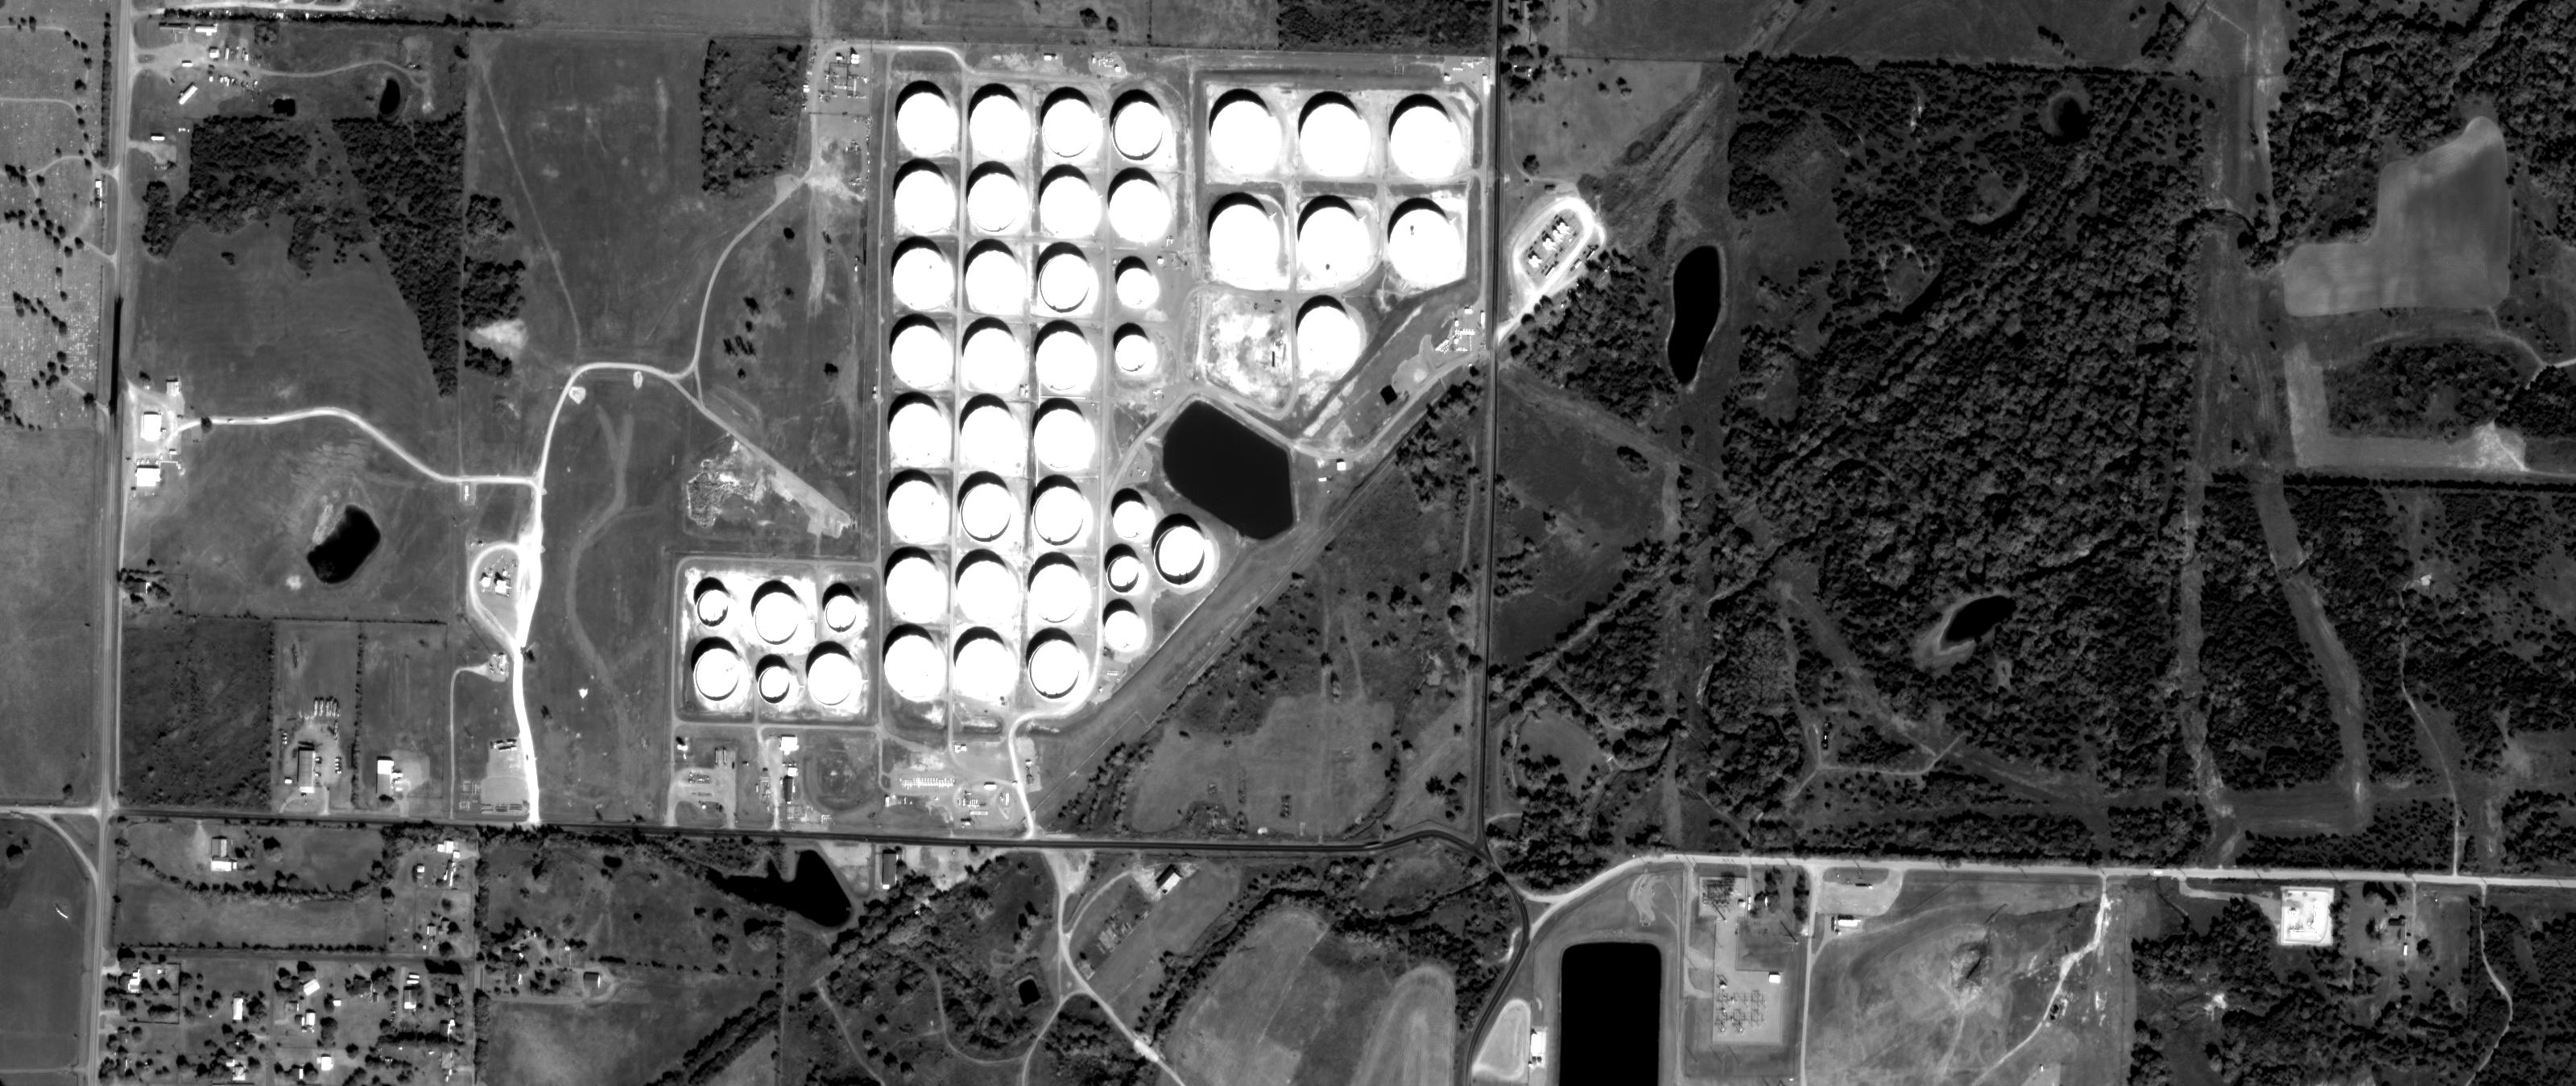
\includegraphics[width=0.9\textwidth]{figures/triplet_1.jpeg}
            \end{subfigure}
 \caption{Two images from SkySat triplets.}
           \label{fig:triplet}
          \end{figure}


    Results from the different methods are compiled in Table \ref{tab:triplet-res}. The images were divided into $3$ tiles of $1000 \times 1000$ pixels.

        \begin{table}[h]
\centering
             \begin{tabular}{|r||c|c|c|}
              \hline
          methods &    tile 1 & tile 2 & tile 3 \\
              \hline
         no correction &    186.9& 82.0& 544.4 \\
             \hline
      (1) & 110.4& 79.5& 63.8\\
       (2) & 110.4& 79.5& 63.8\\
      (3) &  110.4& 79.5& 63.8\\
      (4) &  97.4& 81.0& 43.7\\
      (5) &  75.6& 81.0& 43.7\\
              \hline
            \end{tabular}
                            \caption{Results of pointing error correction on images from the Skysat's triplets.}
             \label{tab:triplet-res}
          \end{table}

     \subsubsection{Results analysis}

We can see that, for all the data, the numerical solutions for the translation are both very close to the analytic solution for the translation (median). For the correction with the rotation and translation, results are quite ambiguous. In fact, wheras the correction with two degree of freedom $(5)$ are always better than the one with only one $(4)$, the correction it-self is sometimes better than the translation only and sometimes a lot worse. For example, on the images from the videos, $(4)$ and $(5)$ are better on tile $1$ but worse on tile $3$.

\subsection{Matches between tiles}

During our experiments, a critial step in correcting the pointing error is the match of keypoints between tiles. Given the time given, we weren't not able to investigate more generally the matching process in \verb|s2p|, but we focused on a representing example: the pair \verb$s03_20161003T161231Z_pan_d1_0002.tif$ and \verb$s03_20161003T161148Z_pan_d1_0002.tif$, which is shown in figure~\ref{fig_sift_input_pair}.


\begin{figure}[H]
    \centering
    \begin{subfigure}[t]{0.8\textwidth}
        \centering
        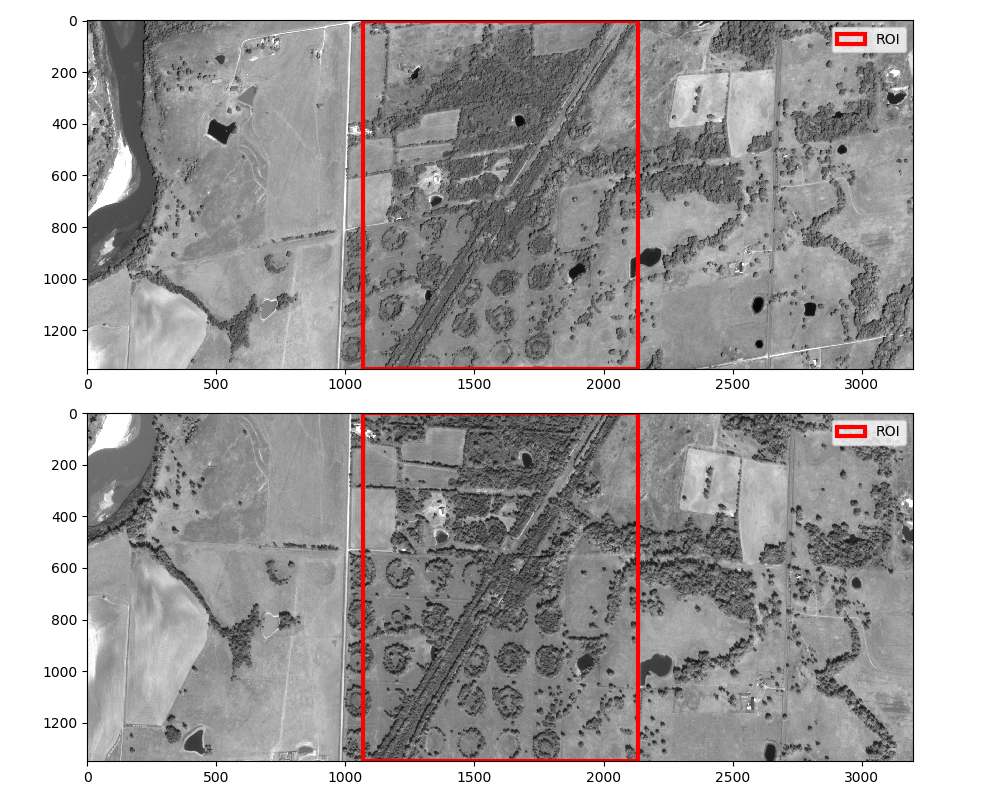
\includegraphics[width = 0.9\textwidth]{ROI_d1_2.png}
        \caption{Input pair to correct. Top: 1Z trace; right: 8Z trace}
    \end{subfigure}%
    ~
    \vfill
    ~
    \begin{subfigure}[t]{0.8\textwidth}
        \centering
        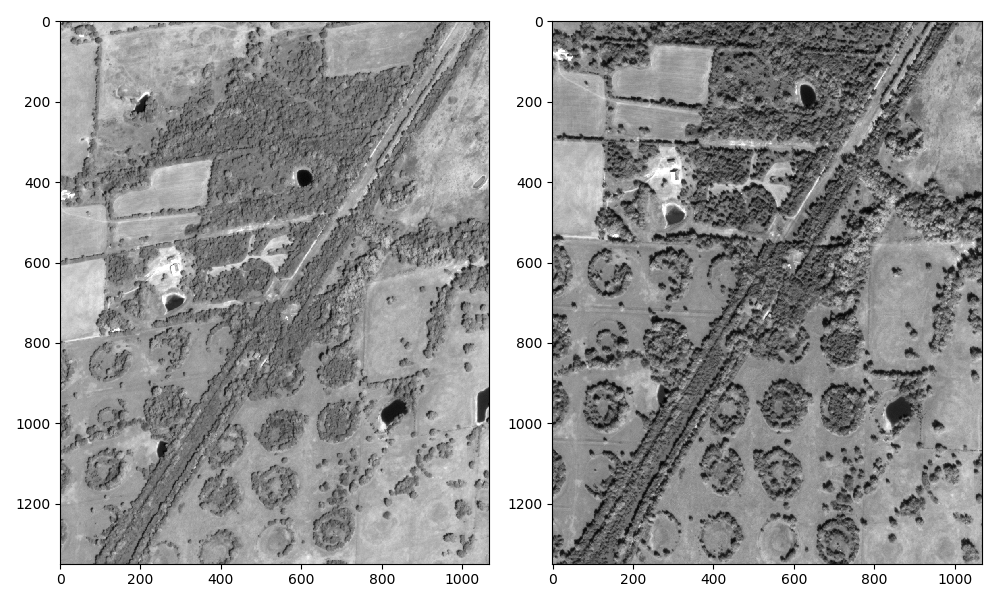
\includegraphics[width = 0.9\textwidth]{ROI_only_match.png}
        \caption{Region of interest. Left: 1Z trace; right: 8Z trace}
    \end{subfigure}%
    \caption{Overview of the ROI of the input pair to correct}
    \label{fig_sift_input_pair}
\end{figure}

On this ROI, three different kinds of keypoints were used. First, the native SIFT algorithm of \verb$s2p$ gives the matches presented in figure~\ref{fig_sift_s2p}, without geometric refinment. The keypoints found are completely false and seem to be influenced by boundaries conditions. The native pipeline find 0 match after refinment. Nonetheless, the SIFT algorithm of OpenCV~\cite{opencv_library} show 25 refined matches, presented in figure~\ref{fig_sift_cv} for the same ROI, given a Lowe's ratio of 0.5: meaning that a match is correct if the distance between the keypoints are at most half the distance between a keypoint and his second closest match. The results are still qualitatively bad. Finaly, the ASIFT algorithm of OpenCV~\cite{opencv_library}, adapted from the IPOL ASIFT algorithm~\cite{ipol_asift}, highlights 2256 refined matches, presented in figure~\ref{fig_asift_cv}. The refinment process used is RANSAC, with a quite large reprojection error of 5 pixels. This time the matches look promising.
In fact, the good performance of the ASIFT algorithm can be expected given its invariance to camera axis orientation, which jeopardizes the SIFT results for Planet Data.

\begin{figure}[H]
    \centering
    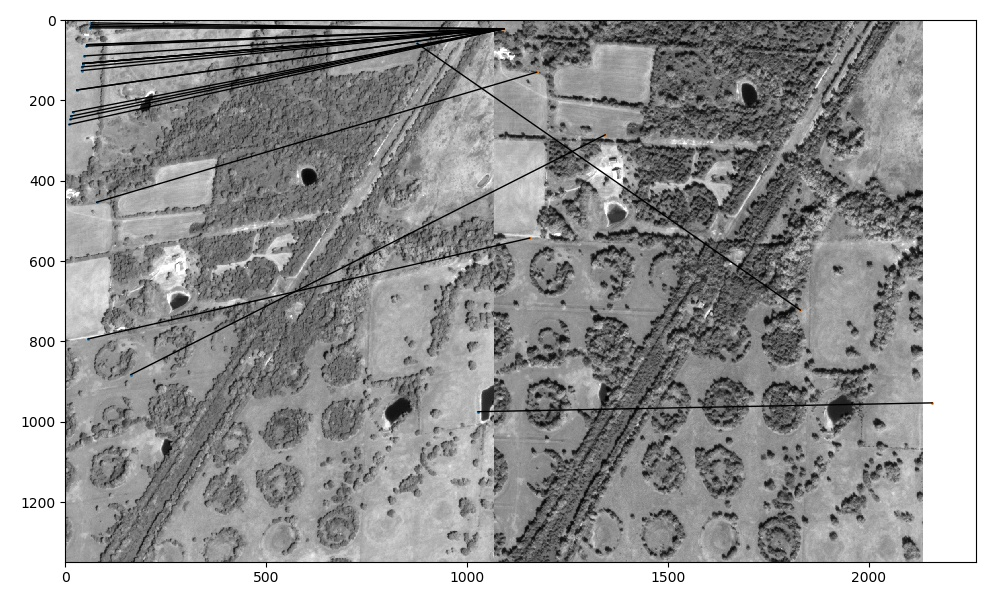
\includegraphics[width = 0.9\textwidth]{sift_s2p_d1_2.jpeg}
    \caption{25 matches found by SIFT on the ROI of interest, implementation from S2P. Without any refinment. Left: 1Z trace; right: 8Z trace}
    \label{fig_sift_s2p}
\end{figure}

\begin{figure}[H]
    \centering
    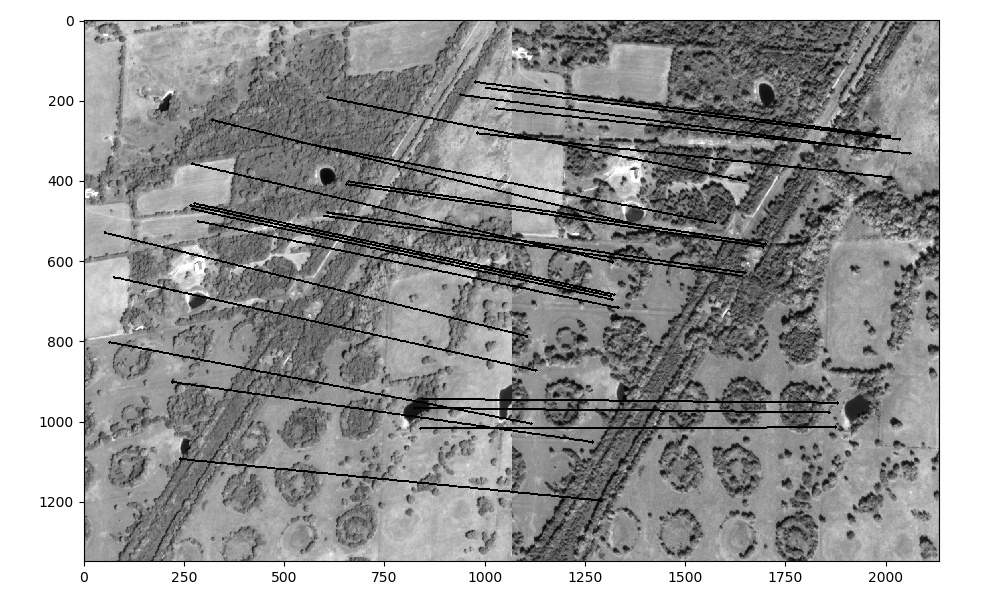
\includegraphics[width = 0.9\textwidth]{sift_cv_d1_2.jpeg}
    \caption{25 refined (Lowe's ratio of $0.5$) matches found by SIFT on the ROI of interest, implementation from OpenCV~\cite{opencv_library}. Left: 1Z trace; right: 8Z trace}
    \label{fig_sift_cv}
\end{figure}

\begin{figure}[H]
    \centering
    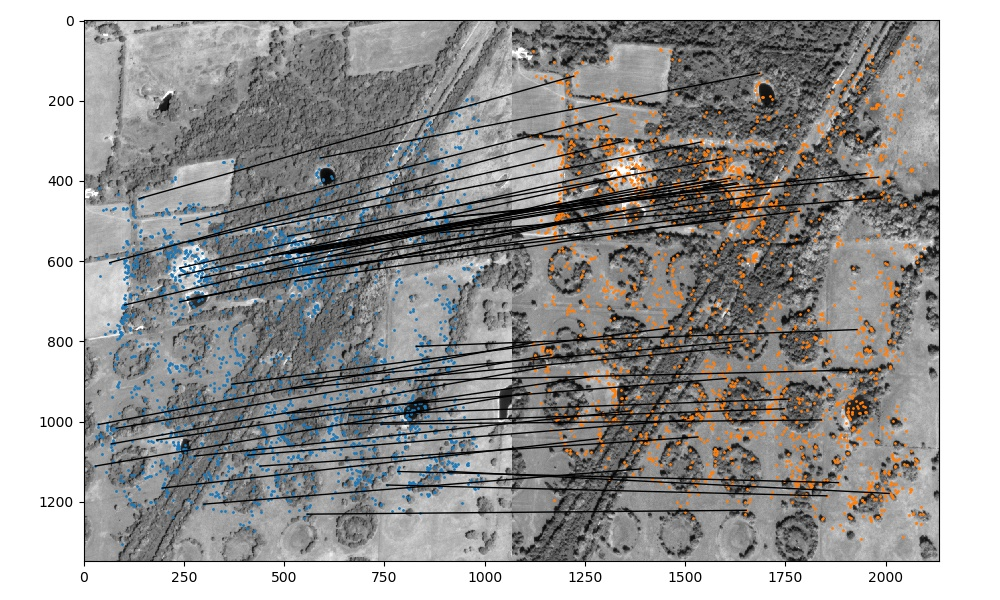
\includegraphics[width = 0.9\textwidth]{asift_cv_d1_2.jpeg}
    \caption{50 first of 2256 refined matches (RANSAC, reprojection error less than 5 pixels) found by ASIFT on the ROI of interest, implementation from OpenCV~\cite{opencv_library}. Left: 1Z trace; right: 8Z trace}
    \label{fig_asift_cv}
\end{figure}

\section{Conclusion and future work}

\subsection{Conclusion}
We propose in this report different ways in order to correct the pointing error which is the consequence of incertitudes in the RPC functions. The pointing error correction is crucial in the \verb|s2p| pipeline as a preprocess for the rectification of the images before triangulation. The methods which were shown here do not seem to improve the performance of the pipeline on Planet's data.\\
Through our tests using s2p, we remarked that the SIFT step were very important for all the next step of the pipeline. In fact without good corrrespondences or not enough, the pipeline were not able to rectify properly the images.
\subsection{Future work}
First more information about the error range of the satellite could be usefull in order to know in which range we have to correct the yaw rotation error. Another idea will be to use ASIFT in the pipeline to be sure that we have enough matches to compute any distance between a point on the epipolar line associated with its match on the other image. Finally, the numeric optimizer seemed to have decent performance and we could use normalization or other degree of freedom to find better pointing error correction.


\newpage

\appendix

\newpage
\section{Mosaic of data}
\label{appen_mosaic}

A mosaic of data gathering the tree traces \verb$s03_20161003T161107Z$, \verb$s03_20161003T161148Z$ and \verb$s03_20161003T161231Z$, respectively refered as 7Z, 8Z, and 1Z are represented for detector 1 (d1) in figure~\ref{fig_mosaic_d1}, for detector 2 (d2) in figure~\ref{fig_mosaic_d2} and for detector 3 in figure~\ref{fig_mosaic_d3}. An important part, which we try to tackle, was to automatically identify pairs and triplets with large overlapping area. This treatment is part of the Planet Post-processing pipeline for Skysat Data~\cite{planet_product} and has not been fully completed, even if a draft in the \verb$geolocalisation$ notebook is available.

\begin{figure}[H]
    \centering
    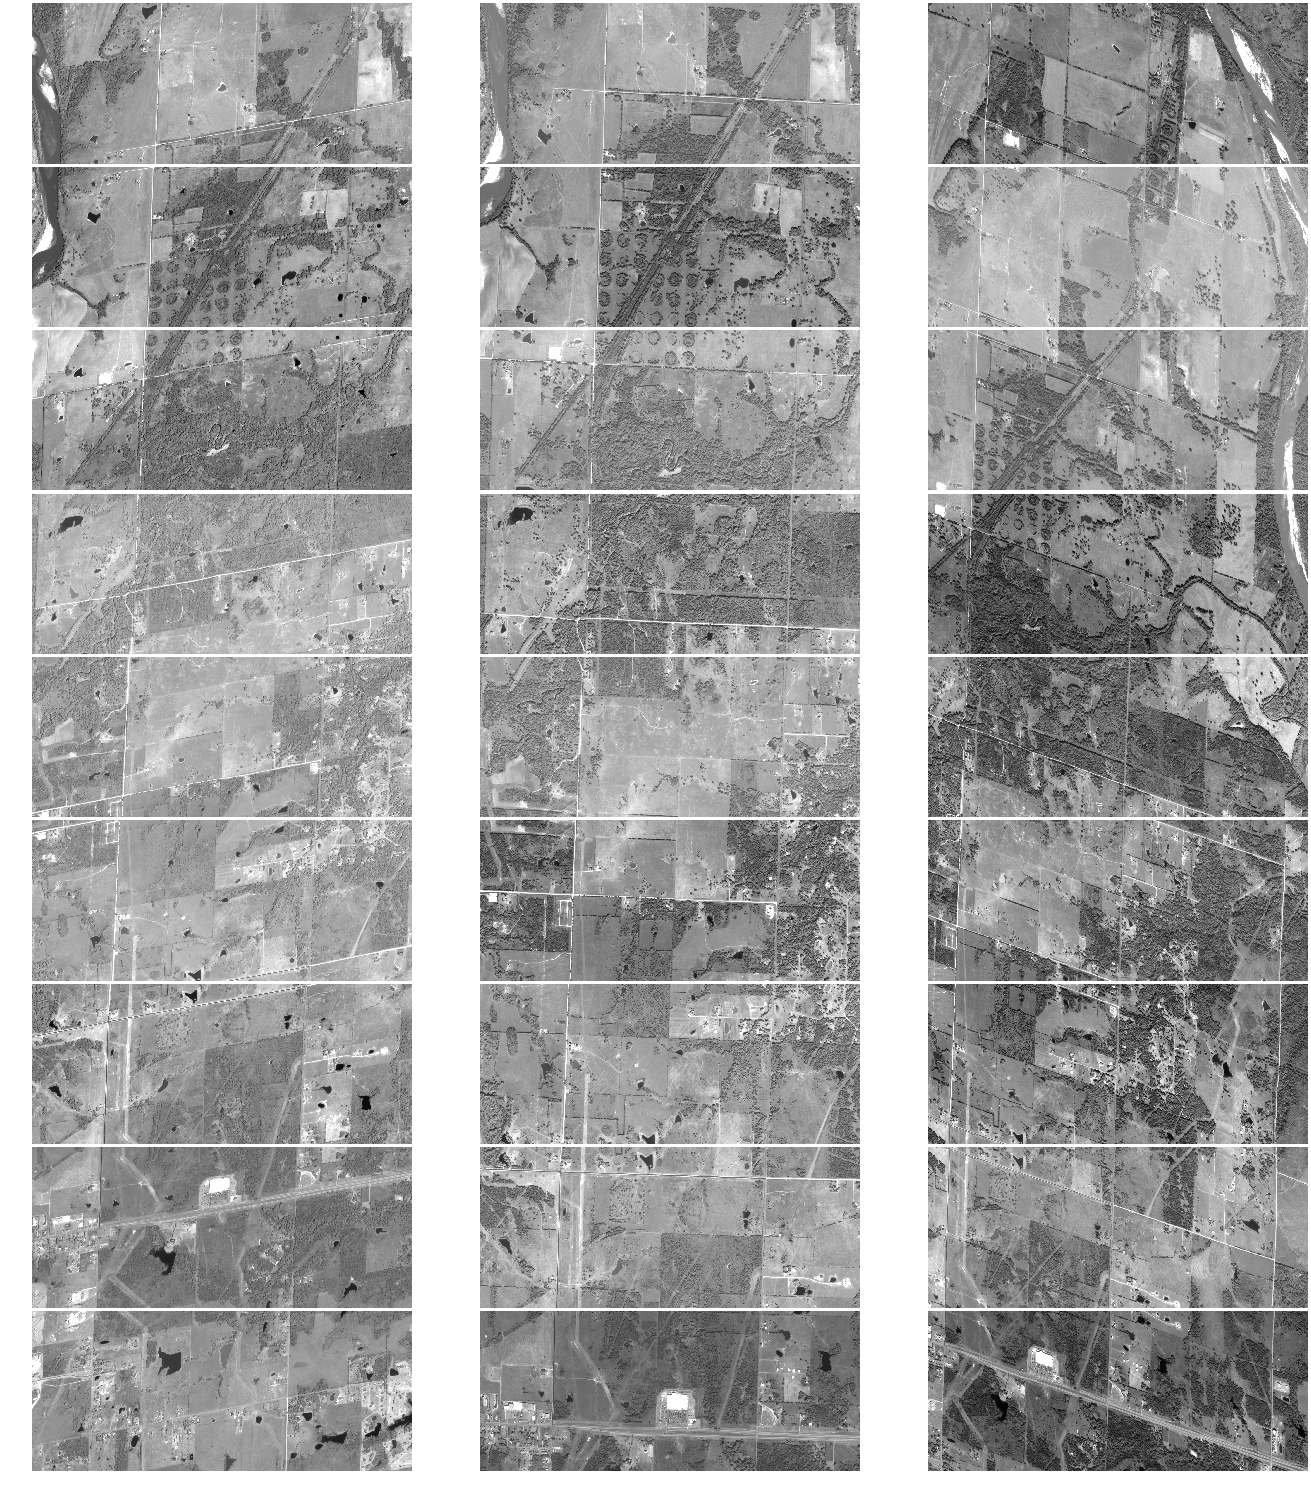
\includegraphics[width = 0.95\textwidth]{d1.png}
    \caption{Mosaic of d1. From left to right: 1Z, 8Z, 7Z}
    \label{fig_mosaic_d1}
\end{figure}

\newpage
\begin{figure}[H]
    \centering
    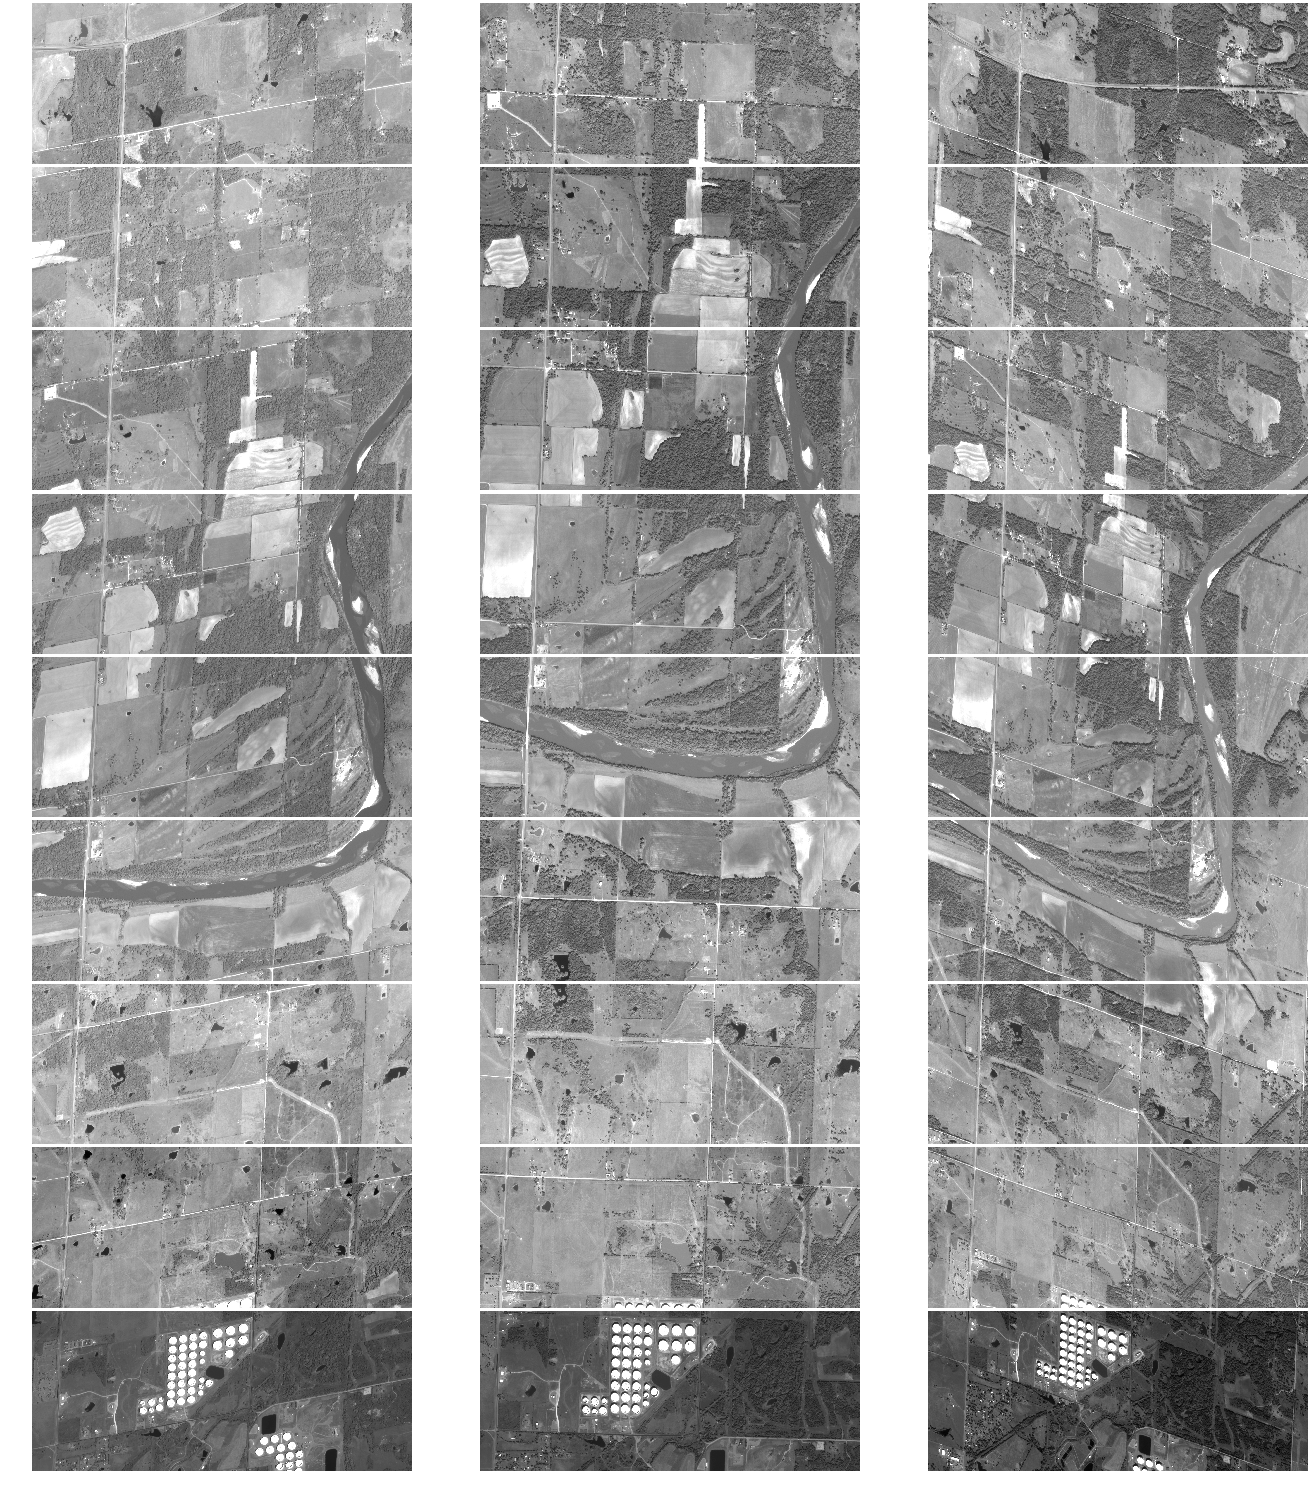
\includegraphics[width = 0.95\textwidth]{d2.png}
    \caption{Mosaic of d2. From left to right: 1Z, 8Z, 7Z}
    \label{fig_mosaic_d2}
\end{figure}

\newpage
\begin{figure}[H]
    \centering
    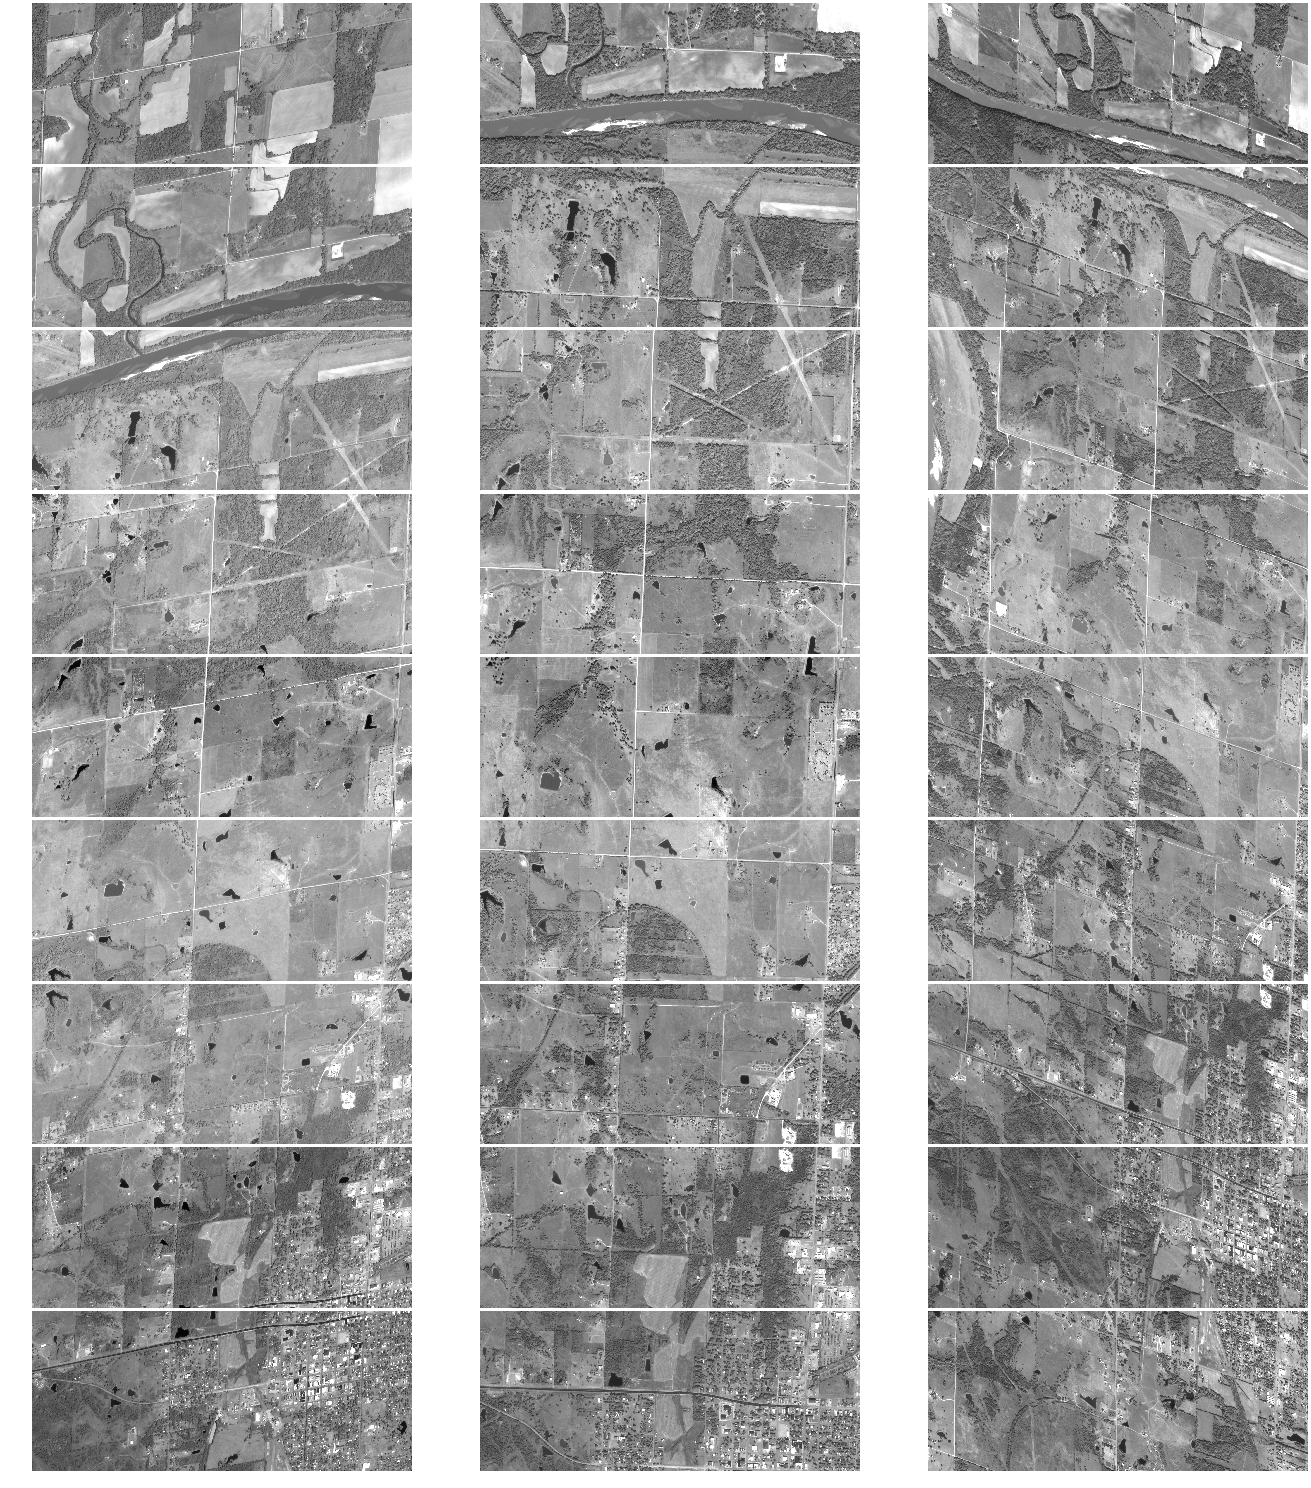
\includegraphics[width = 0.95\textwidth]{d3.png}
    \caption{Mosaic of d3. From left to right: 1Z, 8Z, 7Z}
    \label{fig_mosaic_d3}
\end{figure}


\section{Rotations and translation}

In this part, we consider any point \((x, y) \in \mathbb{R}^2\). As translation and rotation do not commute, we will consider two cases: rotation followed by translation and translation followed by rotation, with \(R\) denoting the rotation of angle \(\theta\) and \(T\) denoting the translation of vector \((t_x, t_y)\). Naming \(f\) the resulting function.

\begin{align*}
    T &=
    \begin{pmatrix}
    1 & 0 & t_x \\
    0 & 1 & t_y \\
    0 & 0 & 1
    \end{pmatrix}
    \\
    R &=
    \begin{pmatrix}
    \cos \theta & -\sin \theta & 0 \\
    \sin \theta & \cos \theta & 0 \\
    0 & 0 & 1
    \end{pmatrix}
\end{align*}


\subsection{Rotation followed by a translation}
This happens when correcting the pointing error first with the rotation.

\begin{align*}
    f(\bm{x}) &= TR\bm{x} \\
    &=
    \begin{pmatrix}
    1 & 0 & t_x \\
    0 & 1 & t_y \\
    0 & 0 & 1
    \end{pmatrix}
    \cdot
    \begin{pmatrix}
    \cos \theta x - \sin \theta y \\
    \sin \theta x + \cos \theta y \\
    1
    \end{pmatrix}
    \\
    &=
    \begin{pmatrix}
    \cos \theta x - \sin \theta y + t_x\\
    \sin \theta x + \cos \theta y + t_y\\
    1
    \end{pmatrix}
\end{align*}

\subsection{Translation followed by a rotation}
This happens when correcting the pointing error first with the translation

\begin{align*}
    f(\bm{x}) &= RT\bm{x} \\
    &=
    \begin{pmatrix}
    \cos \theta & -\sin \theta & 0 \\
    \sin \theta & \cos \theta & 0 \\
    0 & 0 & 1
    \end{pmatrix}
    \cdot
    \begin{pmatrix}
    x + t_x \\
    y + t_y \\
    1
    \end{pmatrix} \\
    &=
    \begin{pmatrix}
    \cos \theta (x + t_x) - \sin \theta (y + t_y)\\
    \sin \theta (x + t_x) + \cos \theta (y + t_y)\\
    1
    \end{pmatrix}
\end{align*}


\bibliographystyle{plain}
\bibliography{biblio}
\end{document}

\end{document}
